\documentclass[preprint,11pt]{elsarticle}
\usepackage[T1]{fontenc}
\usepackage{lmodern}
\usepackage{amsmath,amssymb,booktabs,graphicx,array,longtable,enumitem}
\usepackage[margin=26mm]{geometry}
\usepackage[hidelinks]{hyperref}
\hypersetup{pdftitle={PRISM separates model reliance from context value in multimodal forecasting},pdfauthor={Yanbo Bian; Zhihai Wang}}
\usepackage{xurl}
\usepackage{microtype}
\usepackage{placeins}
\graphicspath{{figures/}}
\newcommand{\prism}{\textsc{PRISM}}
\newcommand{\sag}{\mathrm{SAG}}
\newcommand{\cbtg}{\mathrm{CBTG}}
\newcommand{\mmu}{\mathrm{MMU}}
\newcommand{\fixed}{\mathrm{fixed}}
\newcommand{\retrain}{\mathrm{retrain}}
\journal{Information Fusion}
\setlength{\emergencystretch}{2em}
\renewcommand{\topfraction}{0.90}
\renewcommand{\bottomfraction}{0.90}
\renewcommand{\textfraction}{0.08}
\renewcommand{\floatpagefraction}{0.72}
\begin{document}
\begin{frontmatter}
\title{PRISM separates model reliance from context value in multimodal forecasting}
\author[inst1]{Yanbo Bian}
\ead{2832325140@qq.com}
\author[inst2]{Zhihai Wang\corref{cor1}}
\ead{zhhwang@bjtu.edu.cn}
\affiliation[inst1]{organization={Weihai International College, Beijing Jiaotong University},
  addressline={No. 69 Modern Road, Nanhai New District},city={Weihai},
  postcode={264401},state={Shandong},country={China}}
\affiliation[inst2]{organization={Beijing Jiaotong University},
  addressline={No. 3 Shangyuan Village, Haidian District},city={Beijing},
  postcode={100044},country={China}}
\cortext[cor1]{Corresponding author.}
\begin{abstract}
Text can improve a forecast without showing which cue a model uses or how much information a learning procedure can recover after content disruption. We introduce PRISM (Paired Reliance Interventions with Structured Matching), an evaluation protocol that preserves the observed event process while separating fixed-model reliance from condition-retrained context value. On a natural photovoltaic task, an independent ridge experiment gave alignment gains of 19.65\% for a fixed predictor and 8.97\% after retraining; all twenty additional maps increased fixed-model loss. In twenty generated irregular worlds per mechanism, whole-content permutation detected content dependence in 20/20 worlds for both direction and source targets. Selective edits distinguished the stipulated cues, whereas meaning-preserving paraphrases exposed representation sensitivity. Historical irregular checkpoints showed absolute mean full-dose loss changes below 0.006\% of aligned MSE, with coverage and capability limits, and independent ridge transfer was inconsistent. Separate signal-strength calibration retained ungated null detections of 15\% and 10\%. PRISM links these contrasts to coverage and capability, distinguishing content-position dependence, cue-specific evidence and recoverable context value under a stated learning procedure.

\end{abstract}
\begin{keyword}
Multimodal forecasting \sep Information fusion \sep Content reliance \sep Irregular time series \sep Model evaluation \sep Temporal dependence
\end{keyword}
\end{frontmatter}

\section{Introduction}

Forecasting systems increasingly combine numerical measurements with financial news, operational notes and other textual context. Prediction gains, however, leave the contribution of that context unresolved. A report can carry a directional proposition, identify a source or mark a change in activity through its arrival. Moreover, a fitted model's sensitivity to disrupted content can differ from the information value recovered by retraining. Interpreting contextual forecasts therefore requires separating what the model relies on, which cue it uses and what the learning procedure can recover.

Irregular event schedules make these questions difficult to isolate. Removing text removes its content and occurrence process together. Permuting across entities changes identity and domain; permuting across chronological splits changes evaluation membership. Restricting the permutation preserves those relations but may leave singleton or repeated content unchanged. A small loss difference then has limited reach, while a positive difference can reflect any cue carried by the reassigned content. Both outcomes require the intervention's achieved coverage and the predictor's capability to be made explicit.

Recent benchmarks provide complementary settings for this evaluation. Time-MMD supplies paired numerical and textual series, Time-IMM independently timestamped modalities, and CiK tasks with essential textual information \cite{liu2024timemmd,chang2025timeimm,williams2025context}. Fidel-TS compares original, random and all-zero context on regular tasks \cite{xu2025fidelts}. TimesX extends real-world context diversity and timestamp isolation, and shows that context quality changes forecasting outcomes under a fixed numerical series and prompt \cite{liu2026timesx}. These advances sharpen a complementary question: what does a content intervention establish when the observed event process and forecasting population are held fixed?

Here we introduce \prism{}---Paired Reliance Interventions with Structured Matching---to separate these evaluation questions. The protocol changes text content while retaining entities, split membership, event times, occurrence counts, numerical inputs, targets and forecast windows. It pairs fixed-model and condition-retrained comparisons with achieved coverage, capability evidence and, when a cue is specified, targeted content edits. Structured matching refers to the retained forecast units and event metadata, together with the stated donor restrictions. Tables~\ref{tab:protocol_steps} and~\ref{tab:protocol_worked} make the operations and resulting judgments explicit.

Generated irregular tasks show why this separation matters: whole-content reassignment responds to both a directional proposition and a source cue, whereas selective edits distinguish them. An independent photovoltaic experiment demonstrates the gap between fixed-model reliance and context value after retraining. Historical irregular checkpoints, signal/null calibration, representation alternatives and normalization checks establish where these conclusions remain limited. Together, the comparisons provide an executable route from a content perturbation to the specific inference it supports.

\section{Related work}

\subsection{Contextual forecasting and fusion capability}

Textual context ranges from series metadata and calendar information to event reports and explanatory covariates. The distinctions affect both availability and predictive use. Time-MMD and Time-IMM emphasize complementary temporal settings, whereas MoTime broadens histories and cold-start evaluation \cite{liu2024timemmd,chang2025timeimm,zhou2025motime}. CiK evaluates contexts deliberately required for forecasting, and Fidel-TS provides high-fidelity context controls \cite{williams2025context,xu2025fidelts}. TimesX addresses real-world scale, contamination and context quality; its synthetic-versus-real comparisons also show why constructed tasks cannot establish a real-world model ranking \cite{liu2026timesx}. We use constructed calibration only to assess a diagnostic under known truth.

Forecasting methods increasingly integrate language through mixtures of experts, event-driven reasoning, temporal narratives and constrained auxiliary fusion \cite{lin2026timi,wang2026vot,li2026tats,lee2026cfa}. Their performance comparisons establish capability under their respective designs. \prism{} complements those comparisons by specifying dependence questions for an evaluated function and information-value questions for its learning procedure.

\subsection{Modality reliance and shortcut explanations}

A modality can appear useful while its intended signal remains underused. Shortcut learning, greedy modality learning, gradient imbalance and representation collapse provide mechanisms for such behaviour \cite{geirhos2020shortcut,wu2022greedy,peng2022ogm,chaudhuri2025collapse}. Multimodality can also be redundant conditional on numerical history \cite{zhang2025when}. Ablation studies of language models in forecasting reinforce the need to identify what a language component contributes \cite{tan2024llmuseful}. The content and alignment contrasts measured by \prism{} describe a predictor's response; identifying its optimization mechanism requires additional evidence.

Controlled input changes require a fixed interpretation. Permutation feature importance measures model dependence under a chosen permutation distribution, while conditional importance addresses the effect of dependencies between predictors \cite{fisher2019allmodels,strobl2008conditional}. Continuous-time perturbation methods such as ContiMask explain irregular models in their own temporal setting \cite{moebus2025contimask}. Restricted permutation importance is the closest fixed-model comparator here, and original/random/zero benchmark comparisons already supply content contrasts. A correctly interpreted restricted permutation measures operational reliance under its intervention. Our protocol retains that inference and adds three explicit judgments: coverage identifies the portion of the relation that was tested, targeted edits discriminate stipulated cues, and a separate refit measures adaptation under the changed inputs. Table~\ref{tab:protocol_worked} demonstrates those additions using the same existing contrasts, without attributing unique linguistic meaning to a whole-content effect.

\subsection{Evaluation protocols and dependent uncertainty}

Chronological forecasting can be affected by leakage, inconsistent normalization and mismatched forecast units. Valid time-series evaluation must account for temporal structure \cite{bergmeir2018cv}. Moving-block and stationary bootstrap methods address correlated sequences under their assumptions \cite{kunsch1989block,politis1994stationary}. In our study, training seeds represent algorithmic variation, entities represent application heterogeneity, and repeated windows represent correlated observations. We report those layers explicitly. A post hoc reanalysis of historical test data remains exploratory, even when its new configuration was fixed before that reanalysis.

\section{The PRISM protocol}
\label{sec:protocol}

\subsection{Forecast units and observable invariants}

For entity $i$, an event $e_{ik}=(t_{ik},a_{ik},m_{ik},x_{ik})$ has event time $t_{ik}$, availability time $a_{ik}$, modality $m_{ik}$ and content $x_{ik}$. At forecast origin $q$, eligible inputs satisfy $a_{ik}\leq q$. The text event process contains the entity, split, modality, event and availability times, masks and counts. Content is evaluated conditionally on this observed process; independence between content and process is unnecessary for defining the intervention.

A paired evaluation fixes the numerical observations, target values, target masks, forecast horizons and retained window identifiers. Text content changes at existing eligible positions. Offline Time-IMM loading uses event time as assumed availability time because independent delivery logs are unavailable. This assumption defines the offline experiment and cannot certify availability in an operational deployment.

\subsection{Two distinct evaluation objects}

Let $f=\mathcal{A}(D_{\rm tr})$ denote the aligned predictor selected on validation data, where $\mathcal{A}$ is a specified learning procedure. An input transformation $\mathcal{T}$ changes text content in an evaluation set $D_{\rm te}$, either by a draw from a stated distribution $Q$ or by a specified deterministic edit. Fixed-model evaluation estimates
\begin{equation}
\Delta_{\fixed}(\mathcal{T})=
L(f,\mathcal{T}D_{\rm te})-L(f,D_{\rm te}).
\label{eq:fixed}
\end{equation}
The same checkpoint evaluates every condition. A positive difference indicates sensitivity to the specified content change on the evaluated units. This effect remains defined for a predictor with poor or unassessed forecasting capability. Unless multiple maps are explicitly averaged, the reported effect conditions on the realized $\mathcal{T}$; distributional changes caused by that intervention remain part of its interpretation.

Condition-retrained evaluation instead fits $f_{\mathcal{T}}=\mathcal{A}(\mathcal{T}D_{\rm tr})$, with the corresponding validation condition, and estimates
\begin{equation}
\Delta_{\retrain}(\mathcal{T})=
L(f_{\mathcal{T}},\mathcal{T}D_{\rm te})-L(f,D_{\rm te}).
\label{eq:retrain}
\end{equation}
It evaluates information value achievable by that learning procedure under altered inputs. The exact decomposition
\begin{equation}
\Delta_{\retrain}=\Delta_{\fixed}
+\{L(f_{\mathcal{T}},\mathcal{T}D_{\rm te})-L(f,\mathcal{T}D_{\rm te})\}
\end{equation}
separates the perturbation effect from adaptation under retraining. This is an accounting identity, not a new estimator. The second term can have either sign. We retain the historical retrained results under their original identity and evaluate fixed-model reliance separately.

\begin{figure}[!htbp]
\centering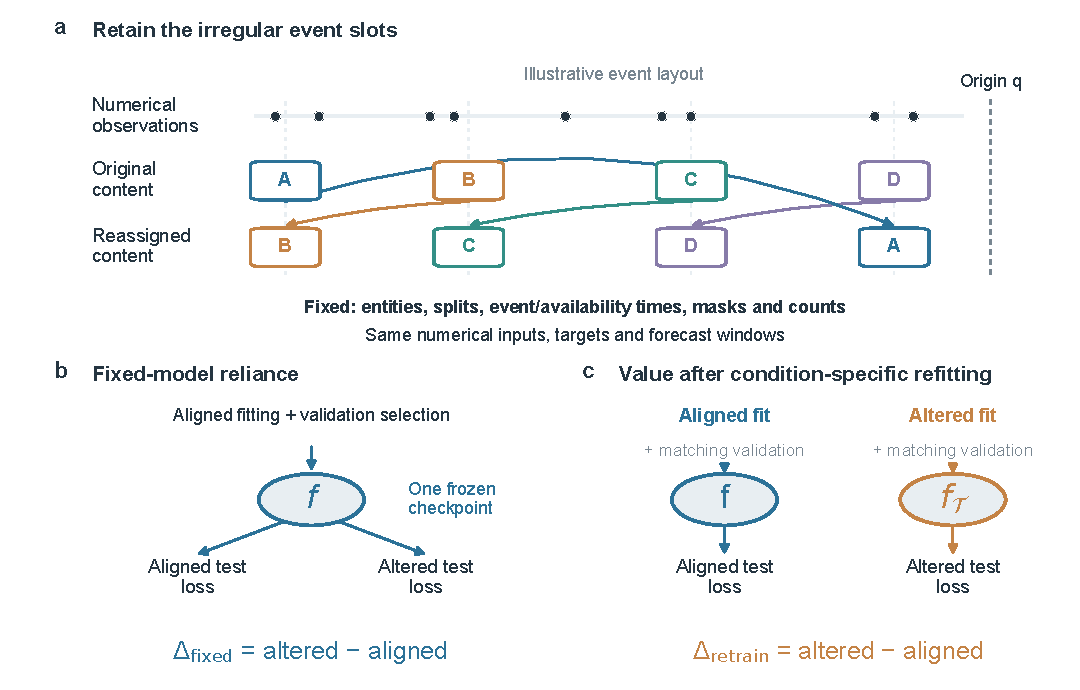
\includegraphics[width=\textwidth]{fig1_estimands}
\caption{Event-preserving content interventions and two evaluation objects. (a) Irregular numerical observations and independently timed text, with content reassigned among retained slots within an allowed entity/split group. Event times, counts, numerical inputs, targets and forecast units stay paired. (b) Fixed-model evaluation retains one aligned checkpoint. (c) Condition-retrained evaluation fits and selects a checkpoint under each altered condition. The event layout is illustrative.}
\label{fig:estimands}
\end{figure}

\subsection{Matched conditions and interpretable contrasts}

Aligned input retains the original content-position pairing. Restricted reassignment draws a bijection according to a stated $Q$. Historical Time-IMM shuffle uses uniform random permutations within entity and chronological split; its full-dose extension uses rejection-sampled uniform derangements. Both generated batches draw uniform nonzero cyclic shifts within each available history. Independent ridge experiments draw uniform nonzero cyclic shifts of ordered content within entity/split, or of the shared within-split report sequence for Fidel-TS. Empty and singleton groups remain unchanged. These laws define different interventions; Table~\ref{tab:capability_overview} reports them alongside the batch evidence.

Time-only input replaces content by a zero vector while preserving occurrence. Numerical-only input removes the text stream, including its event process. Partial-dose replacement and a training-derived neutral representation provide additional controls where the architecture permits them. Retrospective reassignment can use a donor from later in the same test split: recipient slots retain their original eligibility, while donor knowability is a separate question. The resulting experiment measures offline reliance.

With lower loss better, let $A,S,T,N$ denote aligned, shuffled, time-only and numerical-only losses. We report
\begin{equation}
\sag=100\frac{S-A}{S},\qquad
\cbtg=100\frac{T-A}{T},\qquad
\mmu=100\frac{N-A}{N}.
\label{eq:gains}
\end{equation}
Every reported contrast specifies its evaluation object. SAG retains the historical name semantic-alignment gain, but measures an operational content-position contrast under the chosen reassignment. It cannot separate linguistic meaning from source, identity or temporal cues encoded inside content. CBTG compares content with an occurrence-preserving zero marker, so ``beyond timing'' refers only to the retained external event-metadata control and needs sensitivity to that marker. MMU measures complete-stream utility. A separately trained numerical-only model contributes an information-value comparison, rather than a same-checkpoint MMU estimate.

The historical descriptive support rule requires positive SAG and CBTG and at least two of three paired training-seed wins against each control. It is retained as a historical decision rule, not reinterpreted as a significance test. The new fixed-model analyses report paired effect estimates and uncertainty without converting nonsignificance into evidence of absence.

\subsection{Coverage and strength of the intervention}

Let $P$ be a permitted group of $n$ text positions and $\sigma$ a bijection on $P$. We record source-position coverage $1-n^{-1}\sum_j\mathbb{1}\{\sigma(j)=j\}$ and effective representation coverage $1-n^{-1}\sum_j\mathbb{1}\{x_{\sigma(j)}=x_j\}$. These quantities need not agree when representations repeat. A derangement guarantees source-position coverage one for $n\geq2$, but cannot guarantee different content. For $n=1$, the only bijection maps the position to itself, so an entity-preserving alignment test cannot change that group.

We additionally record the time displacement of each donor and recipient and the cosine similarity of their representations. Cosine is a geometric descriptor, not a semantic annotation: a shared representation direction can produce high cosine even when task-relevant propositions differ. Raw-text duplication and controlled proposition changes are assessed separately from vector geometry. Partial-dose experiments report achieved eligible-position coverage, since a requested fraction can be unattainable in small groups.

Stronger controls trade achieved coverage against distributional change. Their interpretation uses the relevant regular-shuffle or neutral-content comparison and, when available, signal/null calibration. A changed entity restriction defines a different intervention and receives a separate report.

\subsection{Capability evidence and protocol execution}
\label{sec:protocol_execution}

Overall predictive capability compares the aligned predictor with a task-appropriate baseline, such as persistence. Incremental content benefit compares it with a matched predictor retaining numerical history and noncontent event timing/counts. Removing the complete text stream instead measures complete-stream utility. Comparator identity, training/validation losses and selection history are recorded for each question, including when no formal screen was applied.

Capability evidence determines how far a functional response informs useful content use, especially when the measured effect is small. The generated batches additionally screen cases using a positive nominal validation lower bound and more than 1\% relative incremental content benefit (Eq.~\ref{eq:validation_content_screen}). This margin is specific to these batches. Dependence measurement itself remains defined without a screen pass; the construct bound is reported as post-selection nominal evidence.

Table~\ref{tab:protocol_steps} gives the execution sequence. Steps 1--4 provide an operational reliance report. Step 5 is optional for that question and necessary for a claim about a named proposition; step 6 extends the report to learning-procedure information value. This structure returns separate judgments when a cue or an unmodifiable pairing remains unresolved.

\begin{table}[!ht]
\centering\small
\setlength{\tabcolsep}{4pt}
\renewcommand{\arraystretch}{1.12}
\caption{Execution and reusable outputs. Required operations produce a conditional reliance measurement and its interpretation context; the two extensions answer additional questions. Recording capability evidence does not require passing a universal gate.}
\label{tab:protocol_steps}
\begin{tabular}{@{}>{\raggedright\arraybackslash}p{0.17\textwidth}>{\raggedright\arraybackslash}p{0.44\textwidth}>{\raggedright\arraybackslash}p{0.34\textwidth}@{}}
\toprule
Operation & Execution & Reusable output\\
\midrule
1. Required: object and units & Fix checkpoint $f$ or learning procedure $\mathcal A$, retained forecast units, availability assumptions, numerical inputs, targets and loss aggregation. & Model/procedure identity, paired unit identifiers and preserved event-process fields.\\
2. Required: intervention & Specify $Q$, permitted donor groups and sampler; record the realized map, changed source positions, changed representations and immutable groups. & Map law and achieved coverage, with donor/recipient displacement and repetition descriptors.\\
3. Required: capability context & Record overall predictive capability and incremental content benefit against named comparators on training/validation data, including selection history or an unassessed status. & Comparator losses and descriptive or screened status, distinct from the test perturbation.\\
4. Required: reliance effect & Pair aligned and reassigned losses at the same fitted state; preserve the unit weighting and report effect uncertainty. Identify the object of any zero, neutral or numerical contrast. & $\Delta_{\fixed}$, its scale and uncertainty; supporting content/stream contrasts. Multiple-map sensitivity is reported separately.\\
5. Proposition extension & Edit the named proposition while retaining the rival cue, and conversely. Use generated truth or task-specific annotations; paraphrase can assess wording sensitivity. & Evidence discriminating the specified cues, or an unresolved proposition-specific interpretation.\\
6. Retraining extension & Fit and select altered-input models using the same learning procedure and corresponding validation condition. & $\Delta_{\retrain}$ and its adaptation term, reported separately from the original function's response.\\
\bottomrule
\end{tabular}
\end{table}

\begin{table}[!ht]
\centering\small
\setlength{\tabcolsep}{3pt}
\renewcommand{\arraystretch}{1.12}
\caption{Worked comparisons using the existing experiments. The second column gives the legitimate reading of aligned/reassigned/zero controls; the remaining columns show what additional operations reveal. Source effects are altered-minus-aligned MSE; SAG and CBTG use Eq.~\ref{eq:gains}. Full uncertainty and population records appear in Tables~\ref{tab:fixed_full}, \ref{tab:construct_full} and~\ref{tab:capability_overview}, and Fig.~\ref{fig:fidel}.}
\label{tab:protocol_worked}
\begin{tabular}{@{}>{\raggedright\arraybackslash}p{0.13\textwidth}>{\raggedright\arraybackslash}p{0.30\textwidth}>{\raggedright\arraybackslash}p{0.28\textwidth}>{\raggedright\arraybackslash}p{0.23\textwidth}@{}}
\toprule
Case & Existing contrasts, correctly interpreted & Additional evidence & Resulting judgment\\
\midrule
CESNET historical checkpoints & Full-derangement intervals span zero. RecAvg has zero-content CBTG 10.476\%. These characterize responses to the specified content controls. & Original shuffle leaves 10/16 source positions unchanged; full derangement leaves 7/16, all in singleton groups (Fig.~\ref{fig:coverage}). Historical screening is not assigned retrospectively. & The fixed-function effect is retained, with seven positions outside the reassignment's reach. The small effect leaves those pairings unresolved.\\
Source-only generated target & Whole rotation raises MSE by 0.770870 and zero content by 0.759390. Restricted permutation already establishes operational dependence on the reassigned content. & Direction flip gives $-0.000228$, with an interval spanning zero; source flip gives $+2.872553$. The directional target shows the complementary response (Fig.~\ref{fig:construct}). & Selective sensitivity supports the stipulated source cue within this generator. The controls distinguish the two cue hypotheses beyond whole-content dependence.\\
Fidel-TS independent ridge & Separately fitted aligned/numerical-only models give 4.89\% utility. Fixed-model SAG is 19.65\% under a shared within-split nonzero report shift. & Condition-retrained SAG is 8.97\% under the same intervention law; validation comparator evidence is descriptive (Table~\ref{tab:capability_overview}). & Refitting partly accommodates changed content. The fitted function's reliance and the learning procedure's information-value contrast require separate estimates.\\
\bottomrule
\end{tabular}
\end{table}


\section{Experimental design}
\label{sec:design}

\subsection{Historical benchmark evidence}

Five Time-IMM datasets cover computing systems (ClusterTrace), network traffic (CESNET), air quality (EPA-Air), financial news (FNSPID) and software development (RepoHealth). Entity-wise chronological splits are 60/20/20 by retained windows. History, forecast horizon and stride are 12 hours for ClusterTrace, seven days for CESNET and EPA-Air, and 31 days for FNSPID and RepoHealth. Numerical scaling uses training observations. All content conditions share window identifiers and targets.

Historical Time-IMM conditions use frozen GPT-2 masked-mean representations and training seeds 53, 67 and 79. The three mechanisms are a selective continuous-time state-space audit subject, official IMM-TSF RecAvg/GR-Add, and official T2V-XAttn/XAttn-Add. The latter two share one pinned codebase and are not independent research lineages. Parameter-matched recurrent, text-only, naive fusion, training-mean, shrinkage and persistence baselines assess simpler explanations. The original implementations and 43 correctness tests remain part of the historical record.

The independent regular Fidel-TS photovoltaic control uses nine Canadian plants and scheduled weather context, with training/validation/test years 2018--2020/2021/2022. It uses the official TGTSF implementation and three paired training seeds. Scheduled future-context availability differs from the historical asynchronous inputs, so this result calibrates the regular task only. The new calibration and external evaluations address distinct settings.

\subsection{New evaluation batches}

The evaluation combines archived checkpoints, known-signal calibration and independent ridge models, followed by construct controls and repeated-map sensitivity. Fixed-checkpoint evaluation reuses 45 aligned states from five Time-IMM datasets, three mechanisms and three training seeds. Eight conditions yield 360 evaluations: aligned input, the original restricted shuffle, four nominal derangement doses (25/50/75/100\%), zero content and a training-derived centroid. Numerical inputs, targets and event metadata remain fixed. Effect intervals use 2,000 paired bootstrap draws with entity resampling and within-entity circular window blocks of lengths 2, 4 and 8. Seeds are paired and averaged within a unit; their variation is reported separately. These exploratory intervals condition on the selected checkpoints, retained entities and realized maps. Archived validation losses against persistence and condition-retrained time-only models appear in Table~\ref{tab:historical_validation}. Formal capability screening remains \emph{Not assessed}; initialized selections are identified separately.

Known-signal calibration tests diagnostic sensitivity under specified truth. Eight EPA-Air event-time templates supply irregular numerical and text schedules. Numerical values, direction-bearing prose, targets and arrival delays are generated independently for each synthetic entity. Each of 20 independently seeded worlds contains 128 training, 32 validation and 128 test entities assigned across the fixed schedules. Four signal strengths $\gamma\in\{0,0.25,0.5,1\}$ share generated inputs within each world, permitting paired dose comparisons at fixed event geometry. Numerical targets are synthetic rather than observed environmental outcomes.

At a query origin, eligible directions are exponentially pooled with a one-day recency scale. The target is $0.8$ times the latest numerical value plus $0.2$ times its history mean, plus $\gamma$ times the variance-normalized eligible direction signal and independent Gaussian noise with standard deviation 0.35. Numerical histories follow an AR(1) process with coefficient 0.985. Independent simulated arrival delay has mean 0.15 days; queries cannot access an unarrived or future event. This generator makes text recoverability explicit while keeping random direction independent of timing and occurrence.

Oracle direction vectors and frozen MiniLM text representations are evaluated separately. Four paired increase/decrease phrasings are used for training and four different pairs for testing. PCA uses training phrases only, and standardized linear predictors are fitted by SGD with L2 regularization $\alpha=0.003$, at most 300 iterations and three fixed optimizer seeds. A numerical/timing comparator, an aligned predictor and a retrained shuffled predictor produce 1,200 fits across the full matrix. These fitting settings are fixed; validation data select neither hyperparameters nor checkpoints in this batch. The primary within-world test is a one-sided paired entity-level $t$ test at 0.05 after averaging optimizer-seed losses within each entity. Across-world detection rates use Wilson intervals. A frozen validation screen for incremental content benefit is applied separately, and both screened and unscreened detection are reported.

\paragraph{Validation screen for incremental content benefit.}
For each generated world, let $\ell^{\rm NT}_{V,e}$ and $\ell^A_{V,e}$ be the numerical/timing and aligned mean validation losses of entity $e$, with windows averaged within entities and optimizer seeds averaged before comparison where applicable. With $n_V=32$, the implemented rule is
\begin{equation}
 \begin{aligned}
 d_e&=\ell^{\rm NT}_{V,e}-\ell^A_{V,e},\qquad
 b_V=\bar d-t_{0.975,31}\frac{s_d}{\sqrt{32}},\\
 r_V&=\frac{\bar\ell^{\rm NT}_V-\bar\ell^A_V}{\bar\ell^{\rm NT}_V}.
 \end{aligned}
 \label{eq:validation_content_screen}
\end{equation}
where $s_d$ is the sample standard deviation of the paired entity differences. The screen requires $b_V>0$ and $r_V>0.01$. It concerns incremental content benefit over a comparator retaining numerical history and event timing. Overall predictive capability is a separate comparison with a task-appropriate forecasting baseline, here persistence for the real-data models. The 1\% margin is a batch-specific screening choice. Failure of either comparison leaves a fixed-model perturbation effect defined, but limits interpreting a small effect as evidence that a capable model ignored available content.

Independent residual-ridge models assess representation and dataset sensitivity, retaining all ten local FNSPID entities and eight EPA-Air entities. Each summary uses the latest four historical notes, with counts and recency retained separately. We compare cached GPT-2 with pinned MiniLM and FinBERT representations \cite{reimers2019sentencebert,minilmmodel,finbertmodel}. Modern encoders use attention-mask token mean pooling, L2 normalization, a 256-token limit and 32-dimensional training-only PCA. FinBERT's classifier head is excluded; its pooled hidden states are not sentence-trained embeddings. Penalties $1,10,100,1000$ are selected on pooled observed-scalar validation MSE. Condition-retrained models have their own validation selection; fixed perturbations retain the aligned checkpoint. Persistence, numerical-only ridge and numerical/timing ridge provide distinct comparator evidence. Their saved validation means address overall prediction and incremental content benefit; no paired validation screen was applied (Table~\ref{tab:ridge_capability_details}).

The same independent modeling route is applied to all nine Fidel-TS plants using numerical history and published weather embeddings. It uses 360 history hours to forecast the next 24 hours at daily origins, the original year splits, and reports whose recorded timestamp is no later than the numerical cutoff. This is a timestamp-restricted published-embedding experiment, not a reproduction of TGTSF or proof of report issuance time. Report validity timestamps are the available metadata; actual publication and arrival timestamps are absent. Shared weather context also precludes treating all plant windows as independent replications.

New configurations and script identities were recorded before their respective scoring batches. The local records are execution freezes, not externally registered studies. The Time-IMM and Fidel-TS historical test sets had already been inspected, whereas the controlled calibration worlds are newly generated. The distinction is retained in the result records.

\subsection{Construct-specific validation and repeated intervention maps}

Construct validation reuses the eight EPA-Air time templates with independent numerical innovations, per-note direction/source signs, sentence assignments, arrival delays and target noise. Twenty worlds each contain 128 training, 32 validation and 128 test entities, with nonoverlapping seven-day histories. Targets add one of three terms to the numerical baseline: variance-normalized recency-pooled direction, its independently generated source counterpart, or training-standardized log available-note count. Noise standard deviation is 0.35. Sixteen directional/source sentences train the representation pipeline, sixteen different directional phrasings provide validation/test inputs and sixteen further phrasings provide paraphrases. The source vocabulary deliberately stays fixed across splits.

Frozen MiniLM pooling, training-only PCA (at most fifteen components) and scaling precede ridge selection from $0.0001,0.01,1,100$ on mean validation entity loss. No latent direction/source readout enters the sentence predictor. The predictor and numerical/timing comparator each undergo validation selection, yielding 480 candidate fits and 120 selected states. The oracle readout directly evaluates the known generator signal without fitting.

The selected models are then screened with Eq.~\ref{eq:validation_content_screen} on the same 32 validation entities used to choose both ridge penalties. Consequently, $b_V$ is a \emph{post-selection nominal lower bound}. The screen is descriptive: its usual two-sided 95\% calculation does not provide an unadjusted 95\% coverage guarantee after this selection. The local freeze fixes the rule but does not remove selection effects. All independent test entities and all predefined control outcomes remain in the reported results, regardless of screening status.

Each aligned predictor evaluates whole permutation, direction flip, source flip, meaning-preserving paraphrase and zero at fixed event slots. In both generated batches, whole permutation is a uniform nonzero cyclic rotation within the current available history, retaining empty/singleton cases. Targeted edits preserve the alternative generated cue. Tests pair mean losses over 128 independently generated test entities within a world; effect intervals use twenty independent worlds, conditional on the same empirical clocks. All predefined cells are reported, with descriptive rejection rates and no universal multiplicity or error-control claim.

The map-sensitivity batch retains the independent aligned ridge states on EPA-Air, FNSPID and Fidel-TS and draws twenty additional maps with seeds 120001--120020. Each entity/split receives an independent uniform nonzero circular shift of ordered content; the same shifts are shared across representations. Fidel shifts the common report sequence within split and shares its map across all nine plants. These draws supplement the original map, without refitting or validation reselection. They report empirical 2.5th--97.5th percentiles and sign counts over maps, separately from population or training uncertainty. Donor timestamps, changed representations, targets and noncontent features are checked for every draw. This batch does not repeat maps for the original neural checkpoints.


\subsection{Aggregation, pairing and uncertainty}

For historical and fixed-checkpoint Time-IMM evaluation, we aggregate squared errors over observed target values within a channel, then average available channel MSEs equally. We report MAE and entity summaries alongside the main metric. Per-window squared-error sums and target counts are retained for paired reanalysis. The independent ridge batch instead pools its observed scalar target errors and separately reports entity-macro MSE; its scores and numerical-window population are not a direct reproduction of the historical feature-macro scores. A position count describes intervention coverage and is not an independent sample count.

New fixed-checkpoint comparisons first pair conditions within each checkpoint and forecast unit. Training-seed effects are described separately from entity and temporal variation. Entity-aware resampling and within-entity temporal blocks preserve the chosen pairing; block-length sensitivity is recorded. All intervals from already inspected Time-IMM test data are exploratory and conditional on the evaluated models and realized reassignment maps. Independent simulated entities and independently generated worlds supply the replication layers for controlled calibration. Supplementary records state the exact resampling scheme for each result.

A nonpositive estimate or an interval spanning zero does not establish practical equivalence. Model capability, effective intervention coverage and representation adequacy condition its interpretation. Any equivalence claim would require a separate, prespecified practical margin. We retain adverse and inconclusive results rather than selecting only settings with a positive content-position effect.

\section{Results}
\label{sec:results}

The results separated two questions: which content cue drove a response, and how that response changed when the predictor was refitted. Generated tasks tested cue discrimination, and Fidel-TS provided a positive natural-data example. Table~\ref{tab:capability_overview} summarizes capability and coverage evidence for the irregular-data cases.

\subsection{Selective content edits discriminate direction from source}

Selective edits distinguished direction from source, despite a whole-permutation response to both cues. Direction signs and arbitrary Cedar/Maple source cues were generated independently in twenty irregular worlds per target mechanism. Targets depended on direction, source or available-note count alone. Each edit retained the alternative cue within the finite test vocabulary (Table~\ref{tab:construct_examples}).

\begin{table}[htbp]
\centering\small
\caption{One paired example from the frozen construct configuration's test and paraphrase templates. Each selective edit changes one stipulated cue while retaining the other; the paraphrase retains both. Targets and the event process remain fixed.}
\label{tab:construct_examples}
\begin{tabular}{@{}>{\raggedright\arraybackslash}p{0.18\linewidth}>{\raggedright\arraybackslash}p{0.78\linewidth}@{}}
\toprule
Condition & Text at the same event slot\\
\midrule
Aligned & We predict that demand will increase in the upcoming interval. Bulletin source: Cedar.\\
Direction flip & We predict that demand will decrease in the upcoming interval. Bulletin source: Cedar.\\
Source flip & We predict that demand will increase in the upcoming interval. Bulletin source: Maple.\\
Paraphrase & An increase in demand is forecast for the interval ahead. Bulletin source: Cedar.\\
\bottomrule
\end{tabular}
\end{table}


Whole permutation, implemented as nonzero cyclic shifts within available histories, detected content-position reliance in 20/20 worlds for both content targets. All these worlds met the post-selection nominal validation screen for incremental content benefit. On the source-only task, whole permutation increased mean MSE by 0.770870 (across-world 95\% interval [0.758012,0.783728]). Direction flip gave $-0.000228$ [$-0.000640$,0.000185], whereas source flip gave 2.872553 [2.840252,2.904853]. The direction-only task showed the complementary pattern: direction flip gave 2.698159 [2.667529,2.728789], and source flip gave $-0.000071$ [$-0.001688$,0.001546]. Selective edits thus identified which stipulated cue drove the dependence detected by whole permutation.

Paraphrasing preserved the generated cues but changed forecasting error. Direction and source probes recovered cue signs in all sixteen test sentences and sixteen paraphrases. Mean MSE fell by 0.030132 on direction targets and 0.005214 on source targets. One direction world and three source worlds nevertheless showed significant degradation. Recoverable cues therefore did not make the predictor invariant to wording.

For timing-only targets, whole permutation gave $-0.000195$ [$-0.000681$,0.000290] and one ungated rejection. No world met the incremental content-benefit screen against the numerical/timing comparator. Its retained event timing/counts defined the process-only boundary for the content test. Complete-stream MMU was not evaluated because no numerical-only comparator was fitted. Table~\ref{tab:construct_full} reports all fifteen predefined outcomes.

\begin{figure}[!htbp]
\centering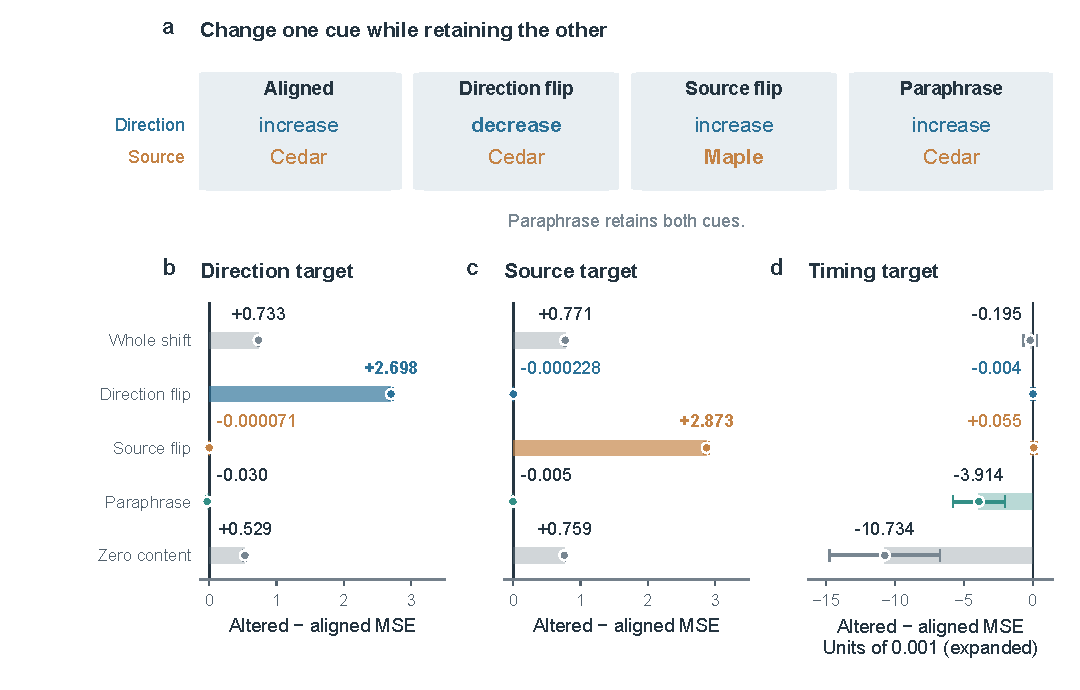
\includegraphics[width=\textwidth]{fig7_construct}
\caption{Selective content edits discriminate the stipulated target cue. (a) Abbreviated direction/source examples show which cue changes; paraphrases change wording while preserving both cues. (b--d) All fifteen fixed-predictor altered-minus-aligned MSE effects for direction, source and timing targets. Points show means and whiskers the saved 95\% $t$ intervals across twenty generated worlds, conditional on shared empirical clocks. Direction and source panels share their scale; the timing axis is expanded in units of 0.001. This contrast concerns the stated cues within the finite generated vocabulary. Table~\ref{tab:construct_full} retains rejection fractions and adverse paraphrase outcomes.}
\label{fig:construct}
\end{figure}


\subsection{Fixed-model reliance and condition-retrained value differ on photovoltaic data}

Refitting reduced the alignment effect in the independent timestamp-restricted Fidel-TS ridge experiment. All nine plants contributed 3,285 daily test windows and 78,840 hourly targets. Numerical-only MSE was 0.191132, compared with 0.181786 for aligned published weather embeddings, giving 4.89\% complete-stream utility. A nonzero cyclic shift of the shared within-split report sequence raised fixed-predictor MSE to 0.226247, giving 19.65\% SAG. Condition-retrained MSE was 0.199692, or 8.97\% SAG, with the same numerical histories and splits. Saved validation comparisons provide descriptive context for overall predictive capability and complete-stream utility (Table~\ref{tab:capability_overview}).

Fixed-shift minus aligned MSE was positive at every plant (0.030509--0.055470); the pooled effect stayed positive across twenty additional maps (Table~\ref{tab:maps}). Plant differences and repeated daily windows share weather context, so they describe heterogeneity without independent replication. The zero-input contrast gave MSE 0.482045 for the same predictor. Median replacement weather-embedding cosine fell from 0.98272 to 0.05801 after training-centroid centering. High raw embedding similarity thus coexisted with a measurable alignment response.

\begin{figure}[!htbp]
\centering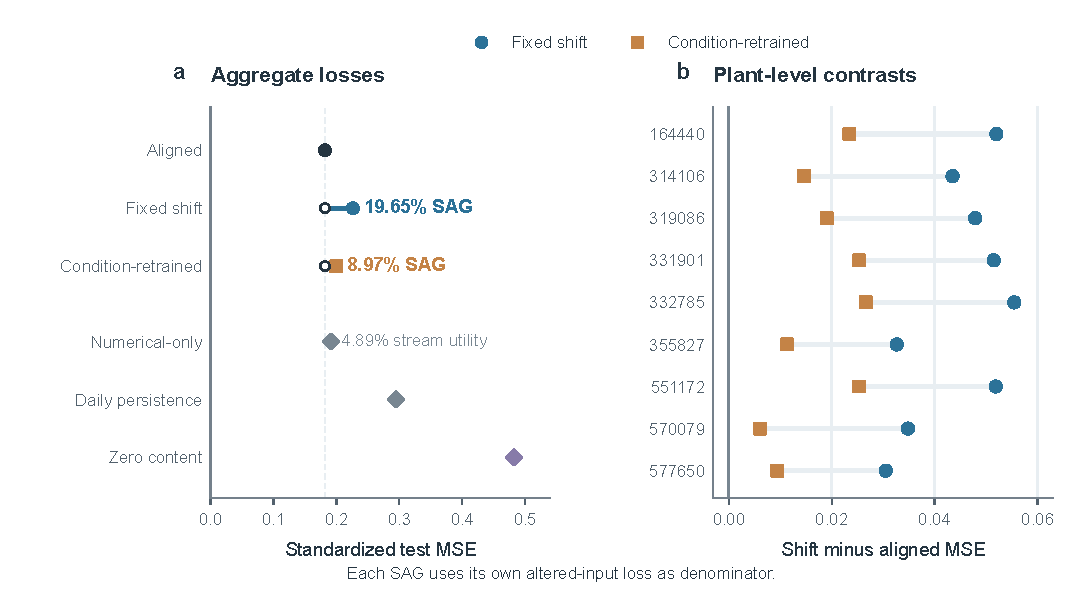
\includegraphics[width=\textwidth]{fig5_fidel}
\caption{Fixed-model reliance and condition-retrained value on the photovoltaic task. (a) Aggregate losses compare the saved input/model conditions. (b) Paired effects connect fixed-shift and retrained-shift contrasts for nine plants. Gains use the corresponding altered-condition MSE as denominator. Plant differences describe heterogeneity under shared weather context, rather than independent-map uncertainty. All 3,285 test windows are retained. Aligned inputs use reports timestamped no later than the cutoff; offline shifts can assign later-dated donors. Issuance and arrival metadata are unavailable.}
\label{fig:fidel}
\end{figure}

\begin{table}[!ht]
\centering\footnotesize
\setlength{\tabcolsep}{4pt}
\caption{Capability evidence and interpretation by batch. Real-data validation comparisons are descriptive; no formal screen was applied. Persistence addresses overall prediction, while a numerical/event comparator addresses incremental content benefit. Fidel's numerical-only comparison measures complete-stream utility. Repeated-map draws retain the aligned model and use the ridge rows' circular-shift families.}
\label{tab:capability_overview}
\begin{tabular}{@{}>{\raggedright\arraybackslash}p{0.20\textwidth}>{\raggedright\arraybackslash}p{0.31\textwidth}>{\raggedright\arraybackslash}p{0.17\textwidth}>{\raggedright\arraybackslash}p{0.25\textwidth}@{}}
\toprule
Evaluation and intervention & Validation evidence and screening status & Achieved intervention & Test evidence\\
\midrule
Historical fixed neural models; restricted random permutation and full derangement & Archived persistence, time-only and aligned validation losses (Table~\ref{tab:historical_validation}). Formal screen: \emph{Not assessed}; 4/45 selections at epoch zero. & Derangement: 56.25\% on CESNET; 100\% elsewhere. & Very small fixed effects; interpretation remains conditional on these checkpoints and maps.\\
Linear known-signal calibration; nonzero within-history rotation & Fixed fitting settings. Incremental-benefit screen: 0/20 null worlds; 20/20 at each nonzero strength, for both representations. & 97.27\% of source positions; 48.52\% of direction values. & Known signal detected in 20/20 worlds per nonzero cell; unscreened null detections 3/20 and 2/20.\\
Construct ridge models; nonzero within-history rotation and cue edits & Same-sample ridge selection and post-selection nominal screen: direction/source 20/20; timing 0/20. & Empty and singleton histories retained; alternative cue preserved in each targeted edit. & Whole-content effects occur for both cues; targeted flips distinguish the generated cue used.\\
EPA-Air ridge; nonzero entity/split circular shift & Persistence validation MSE 1.075034; aligned 0.901160--0.968275. Only FinBERT improves the numerical/timing mean. Formal screen: \emph{Not assessed}. & All selected representations change; latest-four-note summary. & All models lose to test persistence; fixed pooled effects are negative.\\
FNSPID ridge; nonzero entity/split circular shift & Persistence validation MSE 0.648214; aligned 0.673852--0.680205. No overall mean improvement. Formal screen: \emph{Not assessed}. & All selected representations change; latest-four-note summary. & Fixed pooled effects are negative; later test gains do not qualify validation capability.\\
Fidel ridge; nonzero shift of shared split report sequence & Validation numerical 0.221023; aligned 0.208860; persistence 0.350711. Descriptive stream utility 5.50\%. Formal screen: \emph{Not assessed}. & All recipient weather vectors change; one common map across nine plants. & Fixed $\Delta$ MSE +0.044461; retrained +0.017906. The two effects answer different questions.\\
\bottomrule
\end{tabular}
\end{table}

The batches resolve different questions: EPA-Air separates validation improvement from later transfer; FNSPID separates incremental content benefit from overall prediction; Fidel demonstrates complete-stream utility in a regular task. Historical validation losses contextualize fixed-checkpoint effects without adding a screening decision. Full losses and selected epochs appear in Tables~\ref{tab:historical_validation} and~\ref{tab:ridge_capability_details}.


\subsection{Known-signal calibration reveals detection sensitivity and null errors}

Oracle-direction and templated MiniLM predictors detected known signal in 20/20 worlds at each nonzero strength, $\gamma=0.25,0.5,1$. The Wilson 95\% interval for this rate was 83.9--100\%. MiniLM's mean fixed-shift MSE differences were 0.046804, 0.186640 and 0.745574, in strength order. Corresponding across-world 95\% intervals were [0.045030,0.048578], [0.182506,0.190775] and [0.734231,0.756917]. Its held-out direction probe recovered all eight test phrasings, showing recoverability within this controlled vocabulary.

Before screening, null rejection occurred in 3/20 oracle worlds (15\%; Wilson interval 5.2--36.0\%) and 2/20 MiniLM worlds (10\%; 2.8--30.1\%). The descriptive validation screen for incremental content benefit admitted no null world and all tested nonzero worlds. The joint screen-and-detection fraction for null worlds was therefore 0/20, with an upper Wilson bound of 16.1\%. This generator-specific result does not establish a general 5\% error-control guarantee.

Nonzero cyclic shifts within available histories changed 97.27\% of source positions but 48.52\% of direction values. Of test queries, 18.40\% had no available note and 10.41\% had one; all remained in the analysis. Repeated directions preserved some content despite changes in source position. These results describe the evaluated linear pipeline on generated propositions and targets under eight empirical timing templates.

\begin{figure}[!htbp]
\centering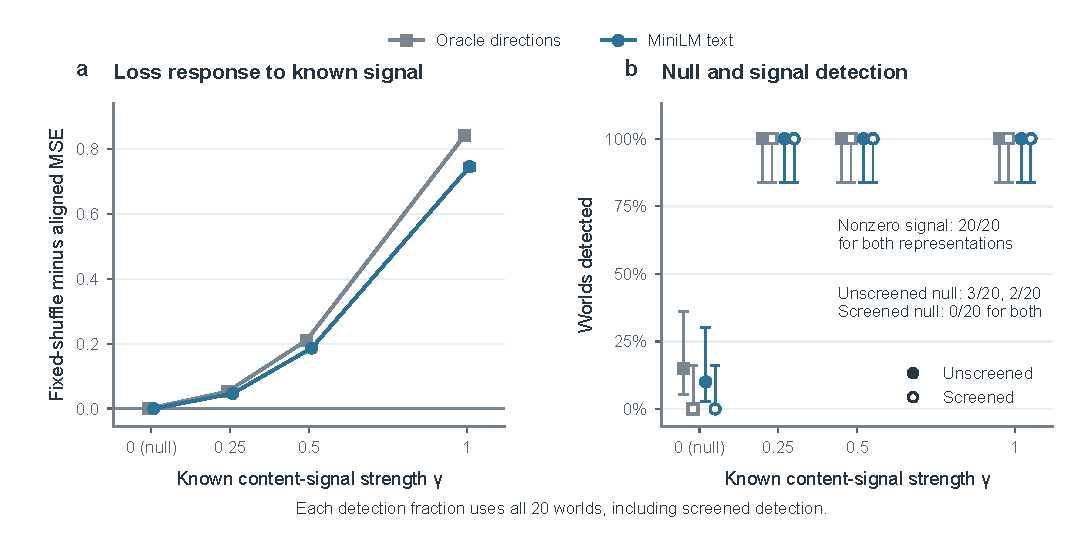
\includegraphics[width=\textwidth]{fig3_calibration}
\caption{Signal-strength calibration under irregular empirical timing templates. (a) Mean fixed-shift minus aligned MSE with saved 95\% $t$ intervals over twenty generated worlds. (b) Unscreened and screened detection fractions with Wilson 95\% intervals. Filled markers show unscreened detection and open markers screened detection; screened detection is the joint screen-and-detection fraction over all twenty worlds. Each within-world test pairs 128 generated entities after averaging three optimizer seeds. Strengths reuse inputs within a world.}
\label{fig:calibration}
\end{figure}

\subsection{Small historical reassignment effects coexist with zero-content sensitivity}

Across fifteen historical dataset/mechanism cells, the largest absolute mean full-derangement change relative to aligned MSE was 0.005868\%, on CESNET cross-attention. Paired block-length 2, 4 and 8 intervals all spanned zero. Four aligned checkpoints selected epoch zero: all three CESNET cross-attention seeds and FNSPID cross-attention seed 53. Tables~\ref{tab:capability_overview} and \ref{tab:fixed_population} provide archived validation context and retained populations; all 45 checkpoints remain formally unassessed for capability screening.

For RecAvg, control-denominator CBTG was 5.119\%, 10.476\%, 10.426\%, 22.726\% and 12.411\% on ClusterTrace, CESNET, EPA-Air, FNSPID and RepoHealth, respectively. The training-content centroid changed MSE by less than 0.005\% of aligned MSE for the same mechanism. Mean zero-content sensitivity thus exceeded sensitivity to content-position pairing. Because zero vectors change representation support as well as information, their loss increase alone does not identify aligned semantic use.

CESNET's nominal doses differed from their achieved interventions. Neither the 25\% nor 50\% dose changed a source position because the per-entity subsets were too small to derange. The 75\% dose changed 12.5\% of all positions, and the full dose changed 56.25\%. These effects concern the selected checkpoints and realized interventions; intervals spanning zero do not establish practical equivalence.

\begin{figure}[!htbp]
\centering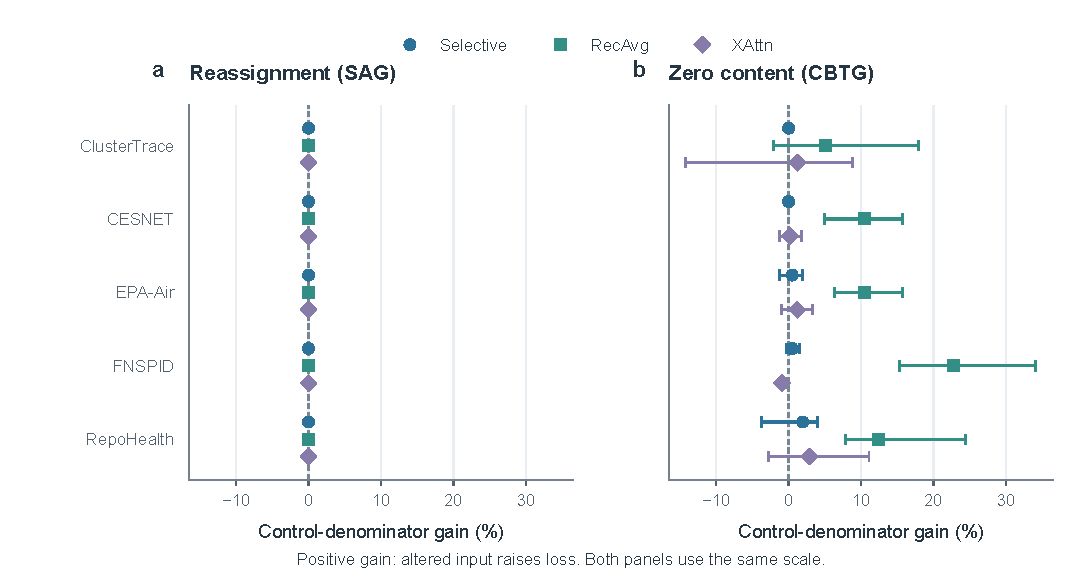
\includegraphics[width=\textwidth]{fig4_fixed_model}
\caption{Same-checkpoint reassignment and zero-content effects across three mechanisms and five datasets. Points show control-denominator $100(L_{\rm altered}-L_{\rm aligned})/L_{\rm altered}$: fixed SAG for full derangement and CBTG for zero input. Bars are the saved paired entity/window-block bootstrap 95\% intervals with block length two; each cell averages three aligned checkpoints. Both panels use the same percentage scale. All fifteen derangement intervals span zero. Full effect records and retained populations appear in Tables~\ref{tab:fixed_full} and~\ref{tab:fixed_population}.}
\label{fig:fixed}
\end{figure}

\subsection{Representation geometry and forecasting transfer require separate checks}

\begin{figure}[!htbp]
\centering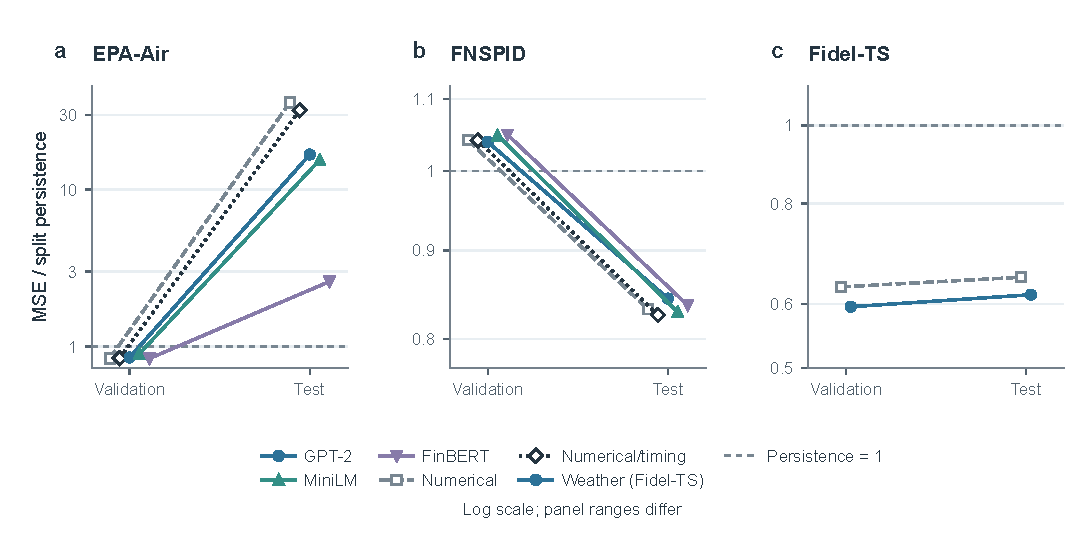
\includegraphics[width=\textwidth]{fig8_transfer}
\caption{Validation comparisons and later test transfer of independent ridge models. Pooled observed-scalar MSE is divided by persistence MSE from the same split; one is the baseline and lower is better. The vertical axis is logarithmic. EPA-Air and FNSPID include numerical, numerical/timing and three aligned text configurations; Fidel-TS includes numerical-only and aligned weather configurations relative to seasonal persistence. Each line connects one validation-selected state across splits. Ratios are descriptive transformations of saved means. Exact losses and penalties appear in Table~\ref{tab:ridge_capability_details}; perturbation contrasts appear in Table~\ref{tab:representations}.}
\label{fig:transfer}
\end{figure}

Validation comparisons and later test transfer are shown in Figure~\ref{fig:transfer}; fixed-model and retrained contrasts are reported in Table~\ref{tab:representations}.


A training-only probe on twelve financial direction sentences allowed MiniLM and FinBERT to classify all twelve differently phrased held-out sentences correctly. The probed direction is therefore recoverable within this vocabulary; forecasting performance requires separate evidence.

Replacement geometry also depends on a shared representation component. On FNSPID, GPT-2's median replacement cosine falls from 0.998964 to 0.188214 after subtracting the training centroid; MiniLM's falls from 0.454059 to 0.142177. On EPA-Air, FinBERT's median falls from 0.768842 to $-0.013962$. Raw cosine can thus be dominated by a shared direction and does not determine whether a task-relevant proposition changed.

On EPA-Air, all three content models improve the validation mean over persistence (1.075034). Only FinBERT improves over numerical/timing ridge (0.901160 versus 0.906853, a descriptive 0.63\% benefit). Every model loses to test persistence (0.751407), including numerical-only and numerical/timing ridge with MSEs of 27.056535 and 24.127104. Negative fixed-shuffle differences therefore accompany poor test-period transfer.

On FNSPID, persistence validation MSE is 0.648214, below numerical ridge (0.675381), numerical/timing ridge (0.675222) and all three content models (0.673852, 0.679578 and 0.680205). GPT-2's 0.20\% mean improvement over numerical/timing ridge thus provides no overall capability advantage. Later gains over test persistence (0.320936) cannot retrospectively qualify validation capability. No formal paired validation screen was applied to these representation comparisons.

Aggregation can reverse the effect's direction. For EPA-Air FinBERT, fixed shuffle reduces scalar-pooled MSE from 1.950746 to 1.945247 but increases entity-macro MSE from 2.388571 to 2.398929. Three of eight entities have a positive alignment point effect. FNSPID has 4/10 such entities for GPT-2, 2/10 for MiniLM and 4/10 for FinBERT. The pooled endpoint therefore need not represent a common entity-level direction.


\subsection{Repeated maps distinguish stable responses from map-sensitive effects}

Fidel's fixed-model response stayed positive under all twenty additional within-split nonzero cyclic shifts. Mean $\Delta$ MSE was 0.047600, the empirical 2.5th--97.5th percentile range was [0.032916,0.064487], and mean map-wise control-denominator SAG was 20.65\%. Positive-map counts for GPT-2, MiniLM and FinBERT were 0/20, 3/20 and 3/20 on FNSPID, and 2/20, 6/20 and 8/20 on EPA-Air. EPA-Air's effect direction thus depended on the map with model states and targets held fixed; Table~\ref{tab:maps} summarizes all seven cells.

Figure~\ref{fig:map_sensitivity} shows intervention-map sensitivity at the selected aligned states, separately from variation across entities or fitted models. Although aligned histories remained timestamp-restricted, offline shifts could assign later-dated donors; Supplementary Section~\ref{sec:map_conditioning} reports their timing fractions and denominators.

\begin{figure}[!htbp]
\centering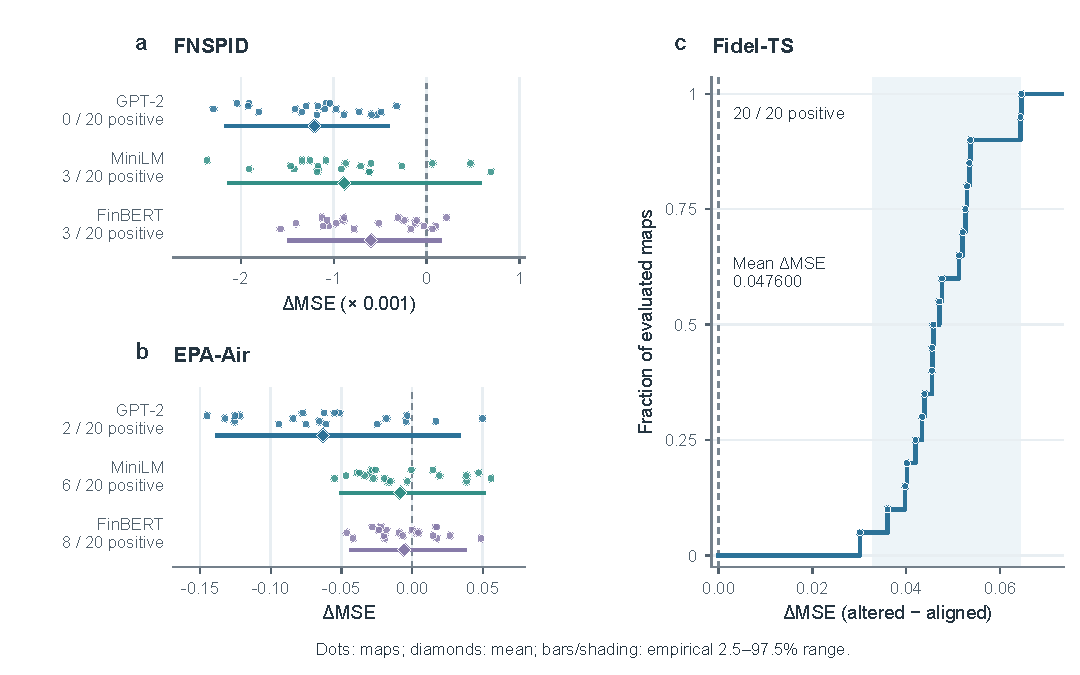
\includegraphics[width=\textwidth]{fig9_map_sensitivity}
\caption{Variation of fixed-model loss effects across the saved nonzero cyclic-shift maps. All 140 altered-minus-aligned MSE effects are retained: three encoder cells on FNSPID, three on EPA-Air and one shared-weather cell on Fidel. Each cell uses twenty maps of the same selected aligned state. (a,b) Encoder-specific effects are shown as strips. (c) Fidel effects are ordered by their empirical cumulative fraction. Zero separates greater altered-input loss from improvement. Bars and shading show saved 2.5th--97.5th percentiles over twenty maps, rather than sampling confidence intervals. Dataset-specific scales reflect different effect magnitudes. The numeric summaries appear in Table~\ref{tab:maps}.}
\label{fig:map_sensitivity}
\end{figure}




\subsection{Historical retrained gains and alignment contrasts diverge}
\label{sec:historical_results}

The earlier TGTSF Fidel-TS control obtains aligned MSE $0.171266\pm0.011401$, shuffled MSE $0.229735\pm0.007647$ and zero-content MSE $0.397442\pm0.280453$ across three seeds. Aligned input improves 25.45\% over shuffle and wins every paired seed against both controls, with substantial training variability in the zero condition. This historical condition-retrained result establishes context value in the specified regular experiment.

The five Time-IMM datasets do not provide stable shared support across the three historical retrained mechanisms. For the selective subject, SAG ranges from $-0.162\%$ on FNSPID to $+0.017\%$ on RepoHealth. Every exploratory selective SAG interval includes zero. EPA-Air nevertheless retains a positive content-beyond-timing contrast and multimodal utility, while RepoHealth multimodal utility is negative. The contrasts therefore distinguish useful occurrence, usable content and original alignment.

FNSPID makes the attribution distinction concrete. The aligned selective candidate improves over the matched multimodal GRU by 1.471\% and naive fusion by 7.972\%, with the required historical paired wins. Separately retrained shuffle and time-only conditions nevertheless improve MSE from 0.268230 to 0.267795 and 0.265485. The historical five-condition gate fails its alignment and content-control conditions. Its rule was internally frozen before original test inspection, rather than publicly registered.

\subsection{Intervention coverage reveals an untestable boundary}
\label{sec:coverage_results}

Reconstructed historical maps retain event metadata, numerical inputs, targets and window identifiers. On CESNET's test set, ten of 16 text positions (62.50\%) retain their original source under the historical shuffle. A derangement reduces the unchanged count to seven (43.75\%), all belonging to singleton groups. Those positions cannot be reassigned while preserving their entity restriction.

For the other four datasets, derangement removes fixed source positions and numerically identical replacements in the evaluated test input. GPT-2 replacement cosine medians remain high; cosine describes geometry rather than semantic equivalence. CESNET's small effect therefore describes a partially altered input, with the singleton pairing outside the intervention's reach. Coverage makes that unresolved portion explicit (Table~\ref{tab:protocol_worked}).

Figure~\ref{fig:coverage}a shows the achieved representation changes, including the nine mutable CESNET positions.

\subsection{Normalization changes the reported metric without improving the forecast}

We isolate a metric effect by evaluating identical physical last-observation persistence under training-only and full-entity normalization. Paired windows require an observed history value for every numerical channel, avoiding a scaler-dependent fallback. Raw squared errors agree within the loader's floating-point tolerance. In contrast, the normalized MSE changes because full-entity standard deviations use future observations and reweight the same physical errors.

\begin{table}[htbp]
\centering\small
\caption{Paired metric sensitivity of an identical physical persistence predictor. Negative changes indicate a lower displayed normalized MSE under full-entity scaling. The forecast does not improve. Windows with an unobserved history channel are excluded from both sides; the same rule and units are retained.}
\label{tab:normalization}
\begin{tabular}{lrrrr}
\toprule
Dataset & Windows used/total & Train-only MSE & Full-entity MSE & Change (\%)\\
\midrule
ClusterTrace & 16/69 & 2.131129 & 0.796068 & $-62.646$\\
CESNET & 12/12 & 1.861666 & 1.831162 & $-1.639$\\
EPA-Air & 39/43 & 1.259575 & 0.719812 & $-42.853$\\
FNSPID & 321/321 & 0.320936 & 0.156170 & $-51.339$\\
RepoHealth & 80/80 & 1.410842 & 1.033575 & $-26.741$\\
\bottomrule
\end{tabular}
\end{table}
The displayed changes range from $-1.639\%$ to $-62.646\%$ (Table~\ref{tab:normalization}), although the largest per-window relative raw squared-error difference is below $6\times10^{-5}$. These persistence windows use the numerical loader and are not claimed to be the identical text-retained population in the historical semantic experiment. Their role is to isolate the numerical scaling effect on the same prediction and target within this paired experiment.


\begin{figure}[!htbp]
\centering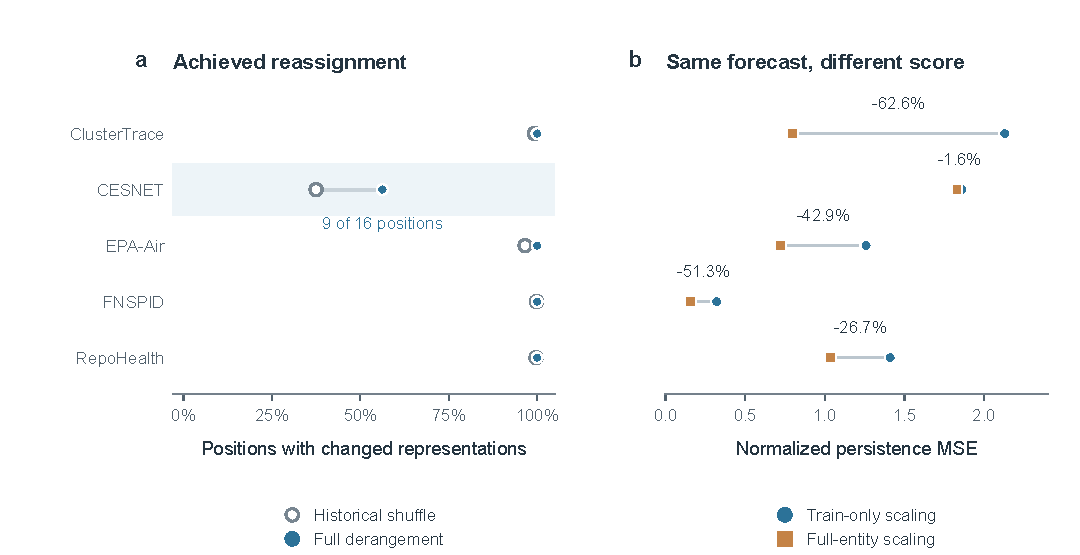
\includegraphics[width=\textwidth]{fig2_coverage}
\caption{Observable boundaries of the paired evaluation. (a) Changed-representation coverage under the original restricted permutation and full derangement on all five historical test sets. CESNET has nine changed positions out of sixteen; seven singleton positions remain beyond the intervention's reach. The counting unit is a retained text position. (b) Identical physical persistence forecasts and eligible windows scored with training-only or full-entity standard deviations. Labels give the percentage change in the displayed normalized MSE, not a predictive improvement. The paired scaling experiment and window rule are detailed in Table~\ref{tab:normalization}.}
\label{fig:coverage}
\label{fig:normalization}
\end{figure}

The historical RecAvg unit-consistency experiment supplies a separate implementation example: changing the time-unit path alters EPA-Air MSE by 0.977\%, larger than its 0.629\% retrained alignment contrast. The new normalization experiment is a metric-sensitivity demonstration with a fixed simple predictor; it is not a learned forecasting improvement. Together, these comparisons show why content contrasts require a matched preprocessing protocol and a stated aggregation rule.

\section{Discussion}

\subsection{Reliance and value support different fusion decisions}

The central distinction is between a fitted model's reliance and the context value available to its learning procedure. A large perturbation effect identifies a vulnerable input relation; refitting tests how much of the loss the procedure can recover under the altered condition. The photovoltaic comparison demonstrates that these quantities can differ substantially. Targeted edits answer a further question: which stipulated cue drives the response? \prism{} makes these questions separately testable rather than assigning them a single semantic score.

The intervention defines the reach of a reliance claim. Strong responses to zero vectors alongside weak responses to reassignment or a training-derived centroid suggest sensitivity to representation support. Singleton groups introduce a complementary boundary: their original content-position relations never enter an entity-preserving reassignment. Coverage and control choice therefore determine which dependence has been tested, including when the measured effect is small.

The construct controls show why whole-content dependence needs a second level of interpretation. A source label is meaningful language, yet dependence on that label differs from dependence on the directional proposition. Selective edits distinguish these stipulated cues, while paraphrase effects expose sensitivity to how the same generated truth is represented. This distinction makes cue-specific evidence useful without elevating it to unrestricted semantic identification.

Capability evidence addresses the value of the evaluated response. Improvement over persistence establishes a different comparison from improvement over a numerical/timing model, while removing the complete text stream measures another quantity. These comparators separate overall prediction, incremental content benefit and complete-stream utility (Table~\ref{tab:capability_overview}). A perturbation effect remains defined when capability is weak or unassessed. Interpreting a small effect as evidence that useful context is absent, however, requires a capable predictor and an effective intervention.


\subsection{From benchmark contrasts to interpretable evidence}

TimesX shows how context quality and realistic benchmark scale shape multimodal performance \cite{liu2026timesx}. \prism{} complements benchmark construction by making the interpretation of a content contrast explicit for a retained forecasting population. Generated tasks test sensitivity and cue discrimination under known truth; natural-data comparisons test operational reliance and transfer. Their distinct roles allow useful dependence evidence to be retained while its cue-specific interpretation remains open (Table~\ref{tab:capability_overview}).

For reuse, each paired effect should carry the predictor or learning-procedure identity, intervention law, achieved coverage and comparator evidence. Targeted controls address a named cue, while retraining addresses recoverable context value (Table~\ref{tab:protocol_steps}). Extending this evaluation to a capable natural irregular-text system with sufficient mutable content is the next application test. The present irregular-data cases identify the coverage and transfer conditions that such a test must resolve.

\subsection{Scope of the evidence}

The evidence supports a conditional evaluation protocol. Historical Time-IMM intervals describe exploratory reanalysis of a shared benchmark lineage with three training seeds and previously inspected test data. Cue discrimination is calibrated within finite generated templates, fixed empirical clocks and the evaluated linear pipelines; extension to the original neural mechanisms or natural language remains untested. The null calibration provides no general 5\% error-control guarantee, and the construct screen is post-selection and descriptive. Chronological downstream splits and recorded event times also leave pretrained contamination and actual report arrival unresolved. Task-specific language controls and availability logs are needed to extend those interpretations.

\section{Conclusion}

\prism{} separates content-position reliance, dependence on a specified cue and context value after retraining. Generated irregular controls demonstrate cue discrimination, and the photovoltaic experiment shows that fixed-model reliance can exceed the alignment value retained after refitting. Coverage and capability evidence define the reach of the remaining contrasts. Together, these components turn a content perturbation into an interpretable evaluation whose conclusion is matched to the tested predictor, learning procedure and intervention.


\section*{Data and code availability}

The manuscript, project adapters, evaluation and plotting code, aggregate reporting inputs and generated-task fitted states are available at \url{https://github.com/bianyanbo44-afk/prism-multimodal-forecasting}. Release \texttt{v0.1.0} provides the generated calibration and construct feature/target arrays, with file hashes and a portable verification entry point. Original Time-IMM and Fidel-TS data and pretrained model weights are acquired from their providers under the applicable source terms; acquisition routes and pinned identities are documented in the repository. Natural-data design matrices, cached report representations and the larger local review/replay package are excluded from the public subset. The editable manuscript archive contains LaTeX, bibliography and figure PDFs. No DOI or journal publication is asserted for this release.

\section*{Declarations}

The study uses public research datasets and explicitly generated calibration data. It introduces no participant recruitment or sensitive personal-data collection. Generative AI assisted research planning, implementation, execution orchestration, result checking, figure construction and drafting. The authors are responsible for verifying the scientific interpretation, sources, author contributions and final submitted version.

\bibliographystyle{elsarticle-num}
\bibliography{references}
\clearpage
\appendix
\section{Execution and evidence identity}

New script and configuration identities are recorded with their result files. Fixed-model evaluation stores each aligned checkpoint hash, 360 per-window SSE/absolute-error/count arrays, and 105 condition comparisons under block lengths 2, 4 and 8. It performs no retraining. The calibration records 20 generated worlds, 1,200 fitted linear models, controlled text events, held-out phrasings, and the entity-level losses. The modern-representation batch stores immutable encoder revisions, caps and token audits, source CSV hashes, validation grids and per-unit predictions. The extension package preserves the original meeting manuscript and historical evidence identities separately.

The fixed-model contrast intervals use entity resampling and paired within-entity circular moving blocks. Seed losses are averaged within the corresponding forecast units; seed variability is separately reported. Original historical intervals instead use their archived seed/within-entity resampling specification. These intervals are not interchangeable and condition on the realized maps. The repeated-map batch reports empirical intervention variation separately, not a forecast-population confidence interval. In controlled calibration, each within-world test averages optimizer seeds and windows at the entity level, then uses a paired $t$ test across 128 generated entities. Across-world intervals treat the 20 independently seeded worlds as the replication units, conditional on the same fixed time templates. Signal strengths reuse a world's generated inputs; no independence across those conditions is assumed.

\section{Availability, intervention and transfer boundaries}

Offline Time-IMM assumes arrival at event time. Calibration uses independently simulated delays and checks the arrival cutoff. The new photovoltaic batch restricts aligned recipient report time but lacks independent issuance metadata. These three availability meanings are retained separately. A fixed-model permutation may transport donor content from elsewhere in the same retrospective test split; it is an offline necessity perturbation and does not claim to be an online implementable missing-data repair. In the photovoltaic derangement, 351 of 3,285 recipient windows (10.685\%) receive content from a donor report whose source timestamp is later than the recipient cutoff. The recorded timestamp-validity flag concerns recipient input slots, not donor knowability. The aligned evaluation and controlled calibration do not use those future donor contents.

The latest-four-note cap applies identically across the three encoders in the independent Time-IMM model and preserves event count/recency features; it does not reproduce the original full-history neural architectures. The independent ridge implementation changes both representation and predictive model relative to that historical study. Its comparisons are within the controlled common ridge scaffold, not an isolated encoder replacement in every original model. All released entities are retained and no test outcome selects them.

\section{Full construct-specific control outcomes}

\begin{table}[htbp]
\centering\small
\caption{All predefined construct/control outcomes on independent test entities. Rejected means an unscreened one-sided paired entity test at 0.05. Effect intervals concern the mean over twenty generated worlds. The descriptive validation screen retains 20/20 direction and source worlds and 0/20 timing worlds; its lower bound is nominal after ridge selection. A 20/20 rejection fraction has Wilson 95\% interval [83.9,100]\%; zero rejections still have upper bound 16.1\%.}
\label{tab:construct_full}
\begin{tabular}{lllll}
\toprule
Target & Control & $\Delta$ MSE & Across-world 95\% interval & Rejected\\
\midrule
Direction & Whole permutation & +0.732964 & [+0.723646, +0.742281] & 20/20\\
Direction & Direction flip & +2.698159 & [+2.667529, +2.728789] & 20/20\\
Direction & Source flip & -0.000071 & [-0.001688, +0.001546] & 0/20\\
Direction & Paraphrase & -0.030132 & [-0.043625, -0.016639] & 1/20\\
Direction & Zero & +0.529420 & [+0.508607, +0.550232] & 20/20\\
Source & Whole permutation & +0.770870 & [+0.758012, +0.783728] & 20/20\\
Source & Direction flip & -0.000228 & [-0.000640, +0.000185] & 1/20\\
Source & Source flip & +2.872553 & [+2.840252, +2.904853] & 20/20\\
Source & Paraphrase & -0.005214 & [-0.010065, -0.000364] & 3/20\\
Source & Zero & +0.759390 & [+0.750211, +0.768568] & 20/20\\
Timing & Whole permutation & -0.000195 & [-0.000681, +0.000290] & 1/20\\
Timing & Direction flip & -0.000004 & [-0.000128, +0.000120] & 0/20\\
Timing & Source flip & +0.000055 & [-0.000151, +0.000261] & 2/20\\
Timing & Paraphrase & -0.003914 & [-0.005802, -0.002026] & 0/20\\
Timing & Zero & -0.010734 & [-0.014727, -0.006740] & 0/20\\
\bottomrule
\end{tabular}
\end{table}

\paragraph{Construct and intervention identities.}
Direction/source signs are independent per note. A direction flip inverts the demand proposition and retains the exact source suffix; a source flip exchanges Cedar/Maple and retains exact proposition text. Paraphrases preserve both latent cues but need not preserve embedding geometry. The validation screen measures incremental content benefit over the numerical/timing comparator by Eq.~\ref{eq:validation_content_screen}. For each model, ridge selection first minimizes mean entity loss over four penalties on the same 32 validation entities subsequently used in that equation. The resulting post-selection nominal lower bound is a descriptive screen, with no unadjusted 95\% coverage claim. Direction and source worlds meet this screen, yet whole permutation alone cannot isolate the directional proposition. Test entities are independently generated and remain in all outcome summaries. No numerical-only comparator was trained for this batch; the available comparator retains numerical and timing features. Full templates, validation candidates and saved predictions are in the local replay package.


\section{Transformation laws and map conditioning}
\label{sec:map_conditioning}

The original fixed-neural batch uses control seed 9103 with entity/split random permutations, derangements and nested dose subsets, shared across architecture/training-seed conditions. Each condition has one realized map and its entity/block bootstrap conditions on that map. The original independent ridge batches also use seed 91801, with a nonzero cyclic rotation per entity/split (the shared report sequence within split for Fidel), rather than unrestricted random derangements. The signal-strength and construct batches use nonzero cyclic shifts within available histories, with empty/singleton histories unchanged; targeted construct edits use deterministic cue mappings. These intervention laws define different perturbation distributions and are not interchangeable.

The repeated ridge maps use the additional twenty seeds 120001--120020, with independent uniform nonzero shifts per permitted group. Source maps are shared across GPT-2/MiniLM/FinBERT for each dataset/draw. The batch retains 140 map-by-cell aggregates, 1,260 entity/plant effect rows and 94,000 donor/recipient timing rows. The minimum and maximum effects, changed-slot counts, donor timing distributions and all per-unit directions are retained, alongside baseline prediction replay, state and target checks. The twenty draws characterize this particular shift distribution; they are not exhaustive permutations or calibrated uncertainty over the original neural models.

\paragraph{Donor timing under offline shifts.}
The fraction of later-dated donors ranges from 1.10\% to 98.90\% of Fidel recipient windows, 33.96\% to 70.96\% of selected FNSPID text slots and 28.36\% to 59.70\% of selected EPA-Air text slots. These denominators differ because the regular batch maps recipient windows and the irregular batches map selected text slots. Aligned inputs remain timestamp-restricted; the shifted conditions measure offline dependence and do not establish deployment-time donor availability.

\paragraph{Supporting prediction replays.}
All 45 historical aligned-checkpoint replays pass, with maximum feature-level MSE discrepancy $1.93\times10^{-8}$. Complete entity losses reconstructed from the signal-strength calibration's saved model states agree with all 102,400 recorded condition-specific entity losses. These checks verify the paired evaluation record and are separate from the evidence for cue discrimination, forecasting capability or natural-data transfer.


\begin{table}[htbp]
\centering\small
\caption{Same-checkpoint loss effects over twenty additional nonzero cyclic-shift maps. Ranges are empirical 2.5th--97.5th percentiles across maps and are not sampling confidence intervals. All rows use scalar-pooled MSE, with predictor state and forecast units fixed.}
\label{tab:maps}
\begin{tabular}{lllll}
\toprule
Dataset & Input & Mean $\Delta$ MSE & Empirical map range & Positive maps\\
\midrule
FNSPID & GPT-2 & -0.001207 & [-0.002175, -0.000401] & 0/20\\
FNSPID & MiniLM & -0.000886 & [-0.002149, +0.000588] & 3/20\\
FNSPID & FinBERT & -0.000600 & [-0.001494, +0.000160] & 3/20\\
EPA-Air & GPT-2 & -0.062968 & [-0.139023, +0.034266] & 2/20\\
EPA-Air & MiniLM & -0.008230 & [-0.050978, +0.051667] & 6/20\\
EPA-Air & FinBERT & -0.005435 & [-0.044129, +0.038321] & 8/20\\
Fidel & Weather & +0.047600 & [+0.032916, +0.064487] & 20/20\\
\bottomrule
\end{tabular}
\end{table}


\section{Saved validation comparisons and their interpretation}
\label{sec:capability_records}

The following tables report existing validation records. Historical checkpoints remain \emph{Not assessed} by a formal screen, and the independent real-data ridge batch did not calculate a paired validation lower bound for screening. The summaries provide comparator context without changing checkpoint selection, introducing test-driven qualifications or excluding outcomes.

\begin{table}[htbp]
\centering\footnotesize
\setlength{\tabcolsep}{4pt}
\caption{Historical selected-model validation MSE and epochs. Persistence is the archived last-observation baseline. Time-only is a separately fitted and validation-selected condition with zero text vectors and retained event metadata. Train-only standardized loss uses the original feature-macro endpoint; stochastic-model losses are means over seeds 53/67/79. Epochs list the aligned selections in that order, with zero indicating initialization. The validation window/query/observed-value counts match within each dataset comparison. All 45 checkpoints retain formal screening status \emph{Not assessed}; retained test populations appear in Table~\ref{tab:fixed_population}.}
\label{tab:historical_validation}
\begin{tabular}{llllll}
\toprule
Dataset & Mechanism & Persistence & Time-only & Aligned & Epochs\\
\midrule
ClusterTrace & Selective & 1.377858 & 1.173743 & 1.175134 & 9/10/9\\
ClusterTrace & RecAvg & 1.377858 & 1.377450 & 1.377379 & 2/1/1\\
ClusterTrace & XAttn & 1.377858 & 1.630176 & 1.604316 & 3/8/12\\
CESNET & Selective & 1.841027 & 1.805790 & 1.805676 & 8/8/8\\
CESNET & RecAvg & 1.841027 & 1.798278 & 1.853441 & 2/3/4\\
CESNET & XAttn & 1.841027 & 1.544668 & 1.531246 & 0/0/0\\
EPA-Air & Selective & 1.919197 & 1.824148 & 1.821315 & 4/4/4\\
EPA-Air & RecAvg & 1.919197 & 1.901226 & 1.902137 & 1/5/9\\
EPA-Air & XAttn & 1.919197 & 2.004410 & 2.022130 & 4/1/6\\
FNSPID & Selective & 0.648214 & 0.598148 & 0.599187 & 4/4/15\\
FNSPID & RecAvg & 0.648214 & 0.648214 & 0.648210 & 1/1/3\\
FNSPID & XAttn & 0.648214 & 1.793357 & 2.057320 & 0/11/1\\
RepoHealth & Selective & 1.527539 & 1.185689 & 1.189478 & 17/15/11\\
RepoHealth & RecAvg & 1.527539 & 1.527807 & 1.525833 & 9/2/1\\
RepoHealth & XAttn & 1.527539 & 1.441968 & 1.427807 & 1/5/5\\
\bottomrule
\end{tabular}
\end{table}

These validation means answer distinct descriptive questions: persistence contextualizes overall prediction, while the condition-retrained time-only model contextualizes content beyond retained occurrence information. An epoch-zero selection identifies a checkpoint state; by itself it does not establish inferiority to persistence. The historical seed average is not an independent sample count or a new confidence estimate.

\begin{table}[htbp]
\centering\footnotesize
\setlength{\tabcolsep}{4pt}
\caption{Saved independent ridge validation and test losses. All losses pool observed standardized scalar targets; $\lambda$ is selected from 1, 10, 100 and 1000 using validation MSE. Numerical/timing adds available-note counts and recency to the numerical design; it supplies the matched comparator for incremental content benefit on Time-IMM. Fidel numerical features include calendar and lag summaries, with no separate weather-event comparator fitted. Validation means are reported after selection and confer no formal screen pass. Test losses contextualize transfer and did not select configurations.}
\label{tab:ridge_capability_details}
\begin{tabular}{lllll}
\toprule
Dataset & Configuration & Selected $\lambda$ & Validation MSE & Test MSE\\
\midrule
EPA-Air & Persistence & -- & 1.075034 & 0.751407\\
EPA-Air & Numerical & 1 & 0.901776 & 27.056535\\
EPA-Air & Numerical/timing & 1 & 0.906853 & 24.127104\\
EPA-Air & GPT-2 aligned & 100 & 0.915482 & 12.580396\\
EPA-Air & MiniLM aligned & 10 & 0.968275 & 11.635062\\
EPA-Air & FinBERT aligned & 100 & 0.901160 & 1.950746\\
FNSPID & Persistence & -- & 0.648214 & 0.320936\\
FNSPID & Numerical & 1000 & 0.675381 & 0.267141\\
FNSPID & Numerical/timing & 1000 & 0.675222 & 0.265127\\
FNSPID & GPT-2 aligned & 1000 & 0.673852 & 0.270960\\
FNSPID & MiniLM aligned & 1000 & 0.679578 & 0.266150\\
FNSPID & FinBERT aligned & 1000 & 0.680205 & 0.268555\\
Fidel-TS & Seasonal persistence & -- & 0.350711 & 0.294942\\
Fidel-TS & Numerical & 100 & 0.221023 & 0.191132\\
Fidel-TS & Aligned weather & 100 & 0.208860 & 0.181786\\
\bottomrule
\end{tabular}
\end{table}

For EPA-Air, all three aligned configurations improve the persistence validation mean, but only FinBERT improves the numerical/timing mean (0.63\%). For FNSPID, none improves the persistence mean; only GPT-2 improves the numerical/timing mean (0.20\%). These point comparisons do not supply the paired lower bound of Eq.~\ref{eq:validation_content_screen}. For Fidel, the aligned validation mean improves by 5.50\% over numerical-only ridge. That comparison measures descriptive complete-stream utility; it does not isolate incremental content benefit with an event-preserving comparator. Seasonal persistence repeats the preceding daily profile, and all plants share weather context.

Time-IMM validation comprises 41 EPA-Air windows and 317 FNSPID windows, with 8,048 and 40,590 observed scalar targets, respectively. Test counts are 43/321 windows and 7,508/41,220 targets. These targets and overlapping windows are scoring units rather than independent replications. Fidel has 3,285 validation and 3,285 test windows, each with 24 hourly targets, across nine plants. Condition-retrained controls have their own validation selection and remain separate from fixed-model effects. Entity-macro results are reported alongside pooled MSE where their directions differ.


\begin{table}[htbp]
\centering\footnotesize
\setlength{\tabcolsep}{4pt}
\caption{Independent ridge representation comparisons, with task baselines shown above each dataset. Loss is pooled observed-scalar standardized test MSE; $\Delta_{\rm fix}=L_{\rm fixed\ shuffle}-L_A$ is the primary effect scale. Fixed shuffle retains the aligned checkpoint, whereas retrained shuffle has its own validation-selected checkpoint. All numerical-adapter windows remain, with at most four historical notes in the content summary. Validation evidence is reported in Table~\ref{tab:ridge_capability_details}; these scores differ from the historical feature-macro endpoint.}
\label{tab:representations}
\begin{tabular}{llllll}
\toprule
Dataset & Representation & Aligned & Fixed shuffle & $\Delta_{\rm fix}$ & Retrained shuffle\\
\midrule
\multicolumn{6}{l}{EPA-Air: persistence 0.751407; numerical/timing 24.127104}\\
EPA-Air & GPT-2 & 12.580396 & 12.429104 & -0.151292 & 7.418856\\
EPA-Air & MiniLM & 11.635062 & 11.599608 & -0.035453 & 8.343223\\
EPA-Air & FinBERT & 1.950746 & 1.945247 & -0.005499 & 17.385432\\
\multicolumn{6}{l}{FNSPID: persistence 0.320936; numerical/timing 0.265127}\\
FNSPID & GPT-2 & 0.270960 & 0.270116 & -0.000844 & 0.267337\\
FNSPID & MiniLM & 0.266150 & 0.264747 & -0.001404 & 0.273117\\
FNSPID & FinBERT & 0.268555 & 0.266923 & -0.001632 & 0.268484\\
\bottomrule
\end{tabular}
\end{table}


\begin{table}[htbp]
\centering\small
\caption{Retained population per aligned checkpoint and historical selection status. Three seeds share each row population, so windows are not multiplied by three. Initialized counts refer to historical best epoch zero. Archived validation comparisons appear in Table~\ref{tab:historical_validation}; no formal capability screen was applied retrospectively.}
\label{tab:fixed_population}
\begin{tabular}{llllll}
\toprule
Dataset & Mechanism & Entities & Windows & Initialized/3 & Formal screen\\
\midrule
ClusterTrace & Selective & 3 & 69 & 0 & Not assessed\\
ClusterTrace & RecAvg & 3 & 69 & 0 & Not assessed\\
ClusterTrace & XAttn & 3 & 69 & 0 & Not assessed\\
CESNET & Selective & 11 & 12 & 0 & Not assessed\\
CESNET & RecAvg & 11 & 12 & 0 & Not assessed\\
CESNET & XAttn & 11 & 12 & 3 & Not assessed\\
EPA-Air & Selective & 8 & 43 & 0 & Not assessed\\
EPA-Air & RecAvg & 8 & 43 & 0 & Not assessed\\
EPA-Air & XAttn & 8 & 43 & 0 & Not assessed\\
FNSPID & Selective & 10 & 321 & 0 & Not assessed\\
FNSPID & RecAvg & 10 & 321 & 0 & Not assessed\\
FNSPID & XAttn & 10 & 321 & 1 & Not assessed\\
RepoHealth & Selective & 4 & 80 & 0 & Not assessed\\
RepoHealth & RecAvg & 4 & 80 & 0 & Not assessed\\
RepoHealth & XAttn & 4 & 80 & 0 & Not assessed\\
\bottomrule
\end{tabular}
\end{table}

Entity resampling in Table~\ref{tab:fixed_full} varies the empirical mixture of these retained entities; the circular blocks vary the sampled window sequences within them. It does not add independent entities. With only three ClusterTrace or four RepoHealth entities, the reported ranges are exploratory descriptions under that resampling scheme, rather than precise coverage guarantees for a wider application population. CESNET has eleven entities but only twelve test windows, a further limit on within-entity temporal information.


\begin{table}[htbp]
\centering\small
\setlength{\tabcolsep}{4pt}
\caption{Full known-signal calibration means over twenty generated worlds after optimizer-seed and entity averaging. Detected means the unscreened within-world one-sided paired test rejects. Zero-strength rows retain false detections. Worlds are independent conditional on eight empirical timing templates; strengths reuse inputs within worlds.}
\label{tab:calibration_full}
\begin{tabular}{llllll}
\toprule
Input & Strength & Aligned & Fixed shuffle & Retrained shuffle & Detected\\
\midrule
Oracle & 0.00 & 0.122392 & 0.122404 & 0.122377 & 3/20\\
Oracle & 0.25 & 0.122397 & 0.175142 & 0.161587 & 20/20\\
Oracle & 0.50 & 0.122405 & 0.332963 & 0.278290 & 20/20\\
Oracle & 1.00 & 0.122432 & 0.963841 & 0.744111 & 20/20\\
MiniLM & 0.00 & 0.122493 & 0.122548 & 0.122522 & 2/20\\
MiniLM & 0.25 & 0.132547 & 0.179351 & 0.164057 & 20/20\\
MiniLM & 0.50 & 0.162285 & 0.348925 & 0.287499 & 20/20\\
MiniLM & 1.00 & 0.280815 & 1.026389 & 0.780037 & 20/20\\
\bottomrule
\end{tabular}
\end{table}
\begin{table}[htbp]
\centering\footnotesize
\setlength{\tabcolsep}{4pt}
\caption{Full-derangement fixed effects: raw feature-macro $\Delta$ MSE and secondary control-denominator SAG. Ranges use the paired block-length-two bootstrap; length-four/eight records are retained separately. These are exploratory uncertainty descriptions under the specified entity/block resampling, conditional on the selected checkpoints and realized maps. Small entity counts constrain their wider-population interpretation (Table~\ref{tab:fixed_population}). Each cell averages three aligned checkpoints; initialized selections and coverage remain visible.}
\label{tab:fixed_full}
\begin{tabular}{lllll}
\toprule
Dataset & Mechanism & $\Delta$ MSE & Fixed SAG (\%) & SAG 95\% range (\%)\\
\midrule
CESNET & RecAvg & $+1.094\times10^{-6}$ & +0.000059 & [-0.000108, +0.000272]\\
CESNET & XAttn & $-8.596\times10^{-5}$ & -0.005868 & [-0.016515, +0.000175]\\
CESNET & Selective & $-5.234\times10^{-7}$ & -0.000029 & [-0.000099, +0.000035]\\
ClusterTrace & RecAvg & $-1.838\times10^{-5}$ & -0.000963 & [-0.004681, +0.001091]\\
ClusterTrace & XAttn & $-2.673\times10^{-5}$ & -0.000781 & [-0.004212, +0.002413]\\
ClusterTrace & Selective & $-3.450\times10^{-6}$ & -0.000186 & [-0.000730, +0.000289]\\
EPA-Air & RecAvg & $-1.891\times10^{-5}$ & -0.001549 & [-0.006282, +0.002163]\\
EPA-Air & XAttn & $+8.205\times10^{-5}$ & +0.005534 & [-0.003253, +0.013631]\\
EPA-Air & Selective & $-2.221\times10^{-5}$ & -0.001848 & [-0.007526, +0.002499]\\
FNSPID & RecAvg & $-1.091\times10^{-7}$ & -0.000034 & [-0.000146, +0.000054]\\
FNSPID & XAttn & $-3.240\times10^{-5}$ & -0.000856 & [-0.005397, +0.003315]\\
FNSPID & Selective & $+3.239\times10^{-6}$ & +0.001208 & [-0.139676, +0.167266]\\
RepoHealth & RecAvg & $+1.960\times10^{-6}$ & +0.000139 & [-0.000157, +0.000757]\\
RepoHealth & XAttn & $+2.007\times10^{-5}$ & +0.000967 & [-0.000751, +0.005386]\\
RepoHealth & Selective & $+9.488\times10^{-7}$ & +0.000077 & [-0.000354, +0.000595]\\
\bottomrule
\end{tabular}
\end{table}

\section{Calibration null behaviour and validation screening}

The unscreened null rejection rates are 3/20 for oracle and 2/20 for MiniLM, with Wilson 95\% intervals [5.24,36.04]\% and [2.79,30.10]\%. The incremental-benefit screen retains no null world, giving screened detections 0/20 for each representation and Wilson interval [0,16.11]\%. These are joint screening-and-detection outcomes over all worlds. No retained null world is available to estimate a conditional rejection rate among screen-positive null worlds.

The screen uses the two-sided 95\% paired-entity lower bound and the more-than-1\% relative improvement rule in Eq.~\ref{eq:validation_content_screen}. Calibration fitting settings are fixed and training-only; the three optimizer seeds are averaged within each of 32 validation entities before the comparison. The construct batch uses the same algebra after ridge selection on those validation entities, so its bound is post-selection nominal and its screening interpretation descriptive. Neither batch establishes general 5\% error control, and the chosen margin may exclude weaker real signals.

\section{Independent model and encoder identities}

MiniLM revision is \nolinkurl{1110a243fdf4706b3f48f1d95db1a4f5529b4d41}; FinBERT revision is \nolinkurl{4556d13015211d73dccd3fdd39d39232506f3e43}. Pooling, maximum token length, cache file hashes and original CSV hashes are in the representation manifest. FinBERT's pinned model card does not supply explicit licence metadata, so the study package includes retrieval instructions rather than redistributing those weights. The two encoders have distinct domain adaptation and pooling provenance.

The independent photovoltaic ridge model selects its penalty from 1, 10, 100 and 1000 using 2021 validation data. Numerical-only features include daily and weekly lag summaries and annual sine/cosine; the content condition adds the most recent published weather-vector summary and training-only PCA. Forecast origin stride is 24 hours; the recorded weather timestamp is exactly at the daily cutoff in this retained population. Neither report issuance nor future-report knowability follows from that equality. Saved validation comparisons appear in Table~\ref{tab:ridge_capability_details}.


\section{Historical evidence retained for comparison}

The following tables retain the original numerical evidence, with its original model, split and seed identities. They are not new experiments. The FNSPID rule was frozen internally before the historical test inspection; its original untouched status applies to that original decision only. New analyses of those test outcomes are exploratory.



\section{Historical experimental and reproducibility details}
\label{app:setup}

\subsection{Time-IMM Data and Training}

The five datasets span computing systems (ClusterTrace), network traffic (CESNET), air quality (EPA-Air), financial news (FNSPID), and software development (RepoHealth). History, horizon, and stride are each 12 hours for ClusterTrace; 7 days for CESNET and EPA-Air; and 31 days for FNSPID and RepoHealth. FNSPID contains 20,826 nonempty notes; median notes per window are 10/13/19 for train/validation/test. CESNET has only 23 training windows across 11 entities and is treated as a low-sample boundary case.

We freeze \texttt{openai-community/gpt2} at commit \texttt{607a30d783df}; mean pooling over the attention mask yields one 768-dimensional vector per note. FNSPID uses maximum token length 320; the maximum observed length is 252. Learned Time-IMM conditions use at most 20 epochs, patience 5, batch size 32, learning rate 0.0015, and weight decay 0.0001. All conditions share seeds, splits, caches, optimization budgets, and validation-based selection.

The selective audit subject maps numerical and text events to 16-dimensional messages, applies learned continuous-time decay to shared/private states, aggregates simultaneous events symmetrically, and updates them through reliability-aware gates. It is an audit instrument, not a proposed Mamba architecture. Public RecAvg/GR-Add and T2V-XAttn/XAttn-Add modules are imported from IMM-TSF commit \texttt{b9e245f2238a}. The attention audit uses text width 128, one head, dropout 0.1, and $\kappa=1.0$; a 768-wide compute pilot was quarantined before the uniform final run. The official TGTSF source is pinned at \texttt{d499d25ee795}; its peak allocated memory is 2.88~GB on an RTX 4060 Laptop GPU.

\subsection{Positive-Control Protocol}

The Canada photovoltaic task uses 360 history hours to forecast 24 hours. Daily window starts produce 9,729 training, 3,285 validation, and 3,285 test examples across nine plants. Per-plant scaling uses training data only. TGTSF trains with AdamW, batch 256, learning rate 0.0005, at most 10 epochs, patience 3, gradient clipping 1.0, and seeds 53/67/79. Aligned, shuffled, and zero conditions retain seven weather-note slots plus one padding slot through an explicit mask.

\begin{table}[htbp]
\caption{Fidel-TS positive-control MSE by seed.}
\label{tab:fidel-seeds}
\centering
\small
\begin{tabular}{lrrrr}
\toprule
Condition & Mean $\pm$ SD & 53 & 67 & 79 \\
\midrule
Aligned & \textbf{0.171266 $\pm$ 0.011401} & 0.163542 & 0.184360 & 0.165895 \\
Shuffle & 0.229735 $\pm$ 0.007647 & 0.223793 & 0.227050 & 0.238361 \\
Zero & 0.397442 $\pm$ 0.280453 & 0.226916 & 0.721126 & 0.244285 \\
\bottomrule
\end{tabular}
\end{table}

\section{Complete Time-IMM Results}
\label{app:results}

\begin{table}[!htbp]
\caption{Selective-family normalized test MSE (mean $\pm$ sample SD across three seeds). Lower is better.}
\label{tab:selective-full}
\centering
\small
\resizebox{\textwidth}{!}{%
\begin{tabular}{lccccc}
\toprule
Dataset & Numeric & Aligned & Shuffle & Time-only & Naive fusion \\
\midrule
ClusterTrace & 1.851027 $\pm$ .013201 & 1.855864 $\pm$ .045990 & 1.855858 $\pm$ .045984 & \textbf{1.848807 $\pm$ .045440} & 1.891028 $\pm$ .038990 \\
CESNET & 1.817116 $\pm$ .003541 & 1.818135 $\pm$ .002036 & 1.818133 $\pm$ .002037 & 1.818094 $\pm$ .001744 & \textbf{1.787256 $\pm$ .080064} \\
EPA-Air & 1.210852 $\pm$ .000900 & 1.201653 $\pm$ .001182 & 1.201726 $\pm$ .001204 & 1.206320 $\pm$ .002539 & \textbf{1.181144 $\pm$ .016645} \\
FNSPID & 0.267905 $\pm$ .007393 & 0.268230 $\pm$ .015631 & 0.267795 $\pm$ .016069 & \textbf{0.265485 $\pm$ .012080} & 0.291467 $\pm$ .005704 \\
RepoHealth & \textbf{1.149093 $\pm$ .017372} & 1.225356 $\pm$ .086849 & 1.225559 $\pm$ .087316 & 1.229270 $\pm$ .091079 & 1.214531 $\pm$ .009684 \\
\bottomrule
\end{tabular}
}
\end{table}

\begin{table}[!htbp]
\caption{Selective-family shortcut-aware metrics and exact exploratory SAG intervals.}
\label{tab:selective-metrics}
\centering
\small
\begin{tabular}{lrrrr}
\toprule
Dataset & SAG & SAG 95\% interval & CBTG & MMU \\
\midrule
ClusterTrace & $-0.000\%$ & $[-0.0077,\ 0.0048]\%$ & $-0.382\%$ & $-0.261\%$ \\
CESNET & $-0.000\%$ & $[-0.0003,\ 0.0001]\%$ & $-0.002\%$ & $-0.056\%$ \\
EPA-Air & $+0.006\%$ & $[-0.0194,\ 0.0203]\%$ & $+0.387\%$ & $+0.760\%$ \\
FNSPID & $-0.162\%$ & $[-0.6413,\ 0.0682]\%$ & $-1.034\%$ & $-0.121\%$ \\
RepoHealth & $+0.017\%$ & $[-0.0959,\ 0.1040]\%$ & $+0.318\%$ & $-6.637\%$ \\
\bottomrule
\end{tabular}
\end{table}

\begin{table}[!htbp]
\caption{FNSPID per-seed normalized test MSE.}
\label{tab:fnspid-seeds}
\centering
\small
\begin{tabular}{lrrrr}
\toprule
Model & Mean $\pm$ SD & 53 & 67 & 79 \\
\midrule
Numeric matched GRU & 0.270994 $\pm$ .006331 & 0.278281 & 0.267863 & 0.266839 \\
Numeric selective SSM & 0.267905 $\pm$ .007393 & 0.264918 & 0.262474 & 0.276324 \\
Multimodal matched GRU & 0.272236 $\pm$ .006122 & 0.269688 & 0.279220 & 0.267799 \\
Aligned selective SSM & 0.268230 $\pm$ .015631 & 0.283774 & 0.268401 & 0.252514 \\
Naive mean-text fusion & 0.291467 $\pm$ .005704 & 0.290480 & 0.297600 & 0.286320 \\
Text-only GRU & 12.600705 $\pm$ .227987 & 12.412091 & 12.854061 & 12.535963 \\
Selective + shuffle & 0.267795 $\pm$ .016069 & 0.283494 & 0.268512 & 0.251380 \\
Selective + time-only & \textbf{0.265485 $\pm$ .012080} & 0.277018 & 0.266514 & 0.252923 \\
\bottomrule
\end{tabular}
\end{table}

\section{Public-Family and Uncertainty Audits}
\label{app:uncertainty}

\begin{table}[!htbp]
\caption{Official RecAvg/GR-Add audit under consistent and released time-unit variants.}
\label{tab:recavg}
\centering
\small
\begin{tabular}{lrrrrr}
\toprule
Dataset & Aligned consistent & Shuffle & Time-only & Released mixed units & Aligned vs. shuffle \\
\midrule
ClusterTrace & 1.908095 & 1.908020 & 1.909383 & 1.908033 & $-0.004\%$ \\
CESNET & 1.842265 & 1.826834 & 1.852595 & 1.842469 & $-0.845\%$ \\
EPA-Air & 1.220996 & 1.213368 & 1.222664 & 1.209068 & $-0.629\%$ \\
FNSPID & 0.320933 & 0.320935 & 0.320936 & 0.320930 & $+0.0008\%$ \\
RepoHealth & 1.409524 & 1.409896 & 1.407048 & 1.407283 & $+0.026\%$ \\
\bottomrule
\end{tabular}
\end{table}

\begin{table}[!htbp]
\caption{Frozen T2V-XAttn/XAttn-Add audit. Seed wins are aligned wins against shuffle/time-only.}
\label{tab:xattn}
\centering
\small
\begin{tabular}{lrrrrcc}
\toprule
Dataset & Aligned & Shuffle & Time-only & Aligned vs. shuffle & Seed wins & Support \\
\midrule
ClusterTrace & 3.422577 & 3.419326 & 3.394558 & $-0.095\%$ & 1/1 & no \\
CESNET & 1.464911 & 1.464825 & 1.467543 & $-0.006\%$ & 1/2 & no \\
EPA-Air & 1.482479 & 1.483506 & 1.472632 & $+0.069\%$ & 2/1 & no \\
FNSPID & 3.782890 & 3.812364 & 3.343304 & $+0.773\%$ & 2/0 & no \\
RepoHealth & 2.075604 & 2.055707 & 2.072985 & $-0.968\%$ & 0/1 & no \\
\bottomrule
\end{tabular}
\end{table}

The hierarchical moving-block bootstrap uses 10,000 replicates, an outer resampling of the three training seeds, and contiguous within-entity blocks of test windows. Block length 3 is primary, with lengths 1 and 5 as sensitivity checks. The analysis was conducted after the frozen FNSPID decision and is not multiplicity-adjusted.

\section{Source Audit and Reproducibility Checklist}
\label{app:repro}

The source audit pins Time-IMM commit \texttt{e934cef23d52} and IMM-TSF commit \texttt{b9e245f2238a}. The released loader standardizes each entity before its chronological split; the released window builder removes histories with no text even when text is disabled; cached and raw text paths use different timestamp origins; and the released RecAvg path subtracts raw within-window text times from normalized query times. Our controlled path fits scaling on training observations, fixes one retained-window set, anchors text to the first numerical timestamp, and compares query/text time on the same axis. These are observable source behaviors; no claim is made about author intent.

Forty-three automated tests cover event availability, grouped-event symmetry, unchanged counterfactual entities, splits, times, counts, targets, and windows, plus batching, CPU/GPU agreement, explicit masks, and source-adapter behavior. Primary tables are generated from frozen JSON artifacts. The artifact records dataset/split identifiers, encoder and upstream commits, maximum length and pooling, cache hashes, all three seeds, model selection rules, internally frozen decisions, per-seed values, and figure source data. Raw benchmark data are excluded.



\end{document}
